\chapter{Tervezés} \label{chapter3}

\section{A szoftver architektúrája}

\begin{figure}[!h]
	\centering
        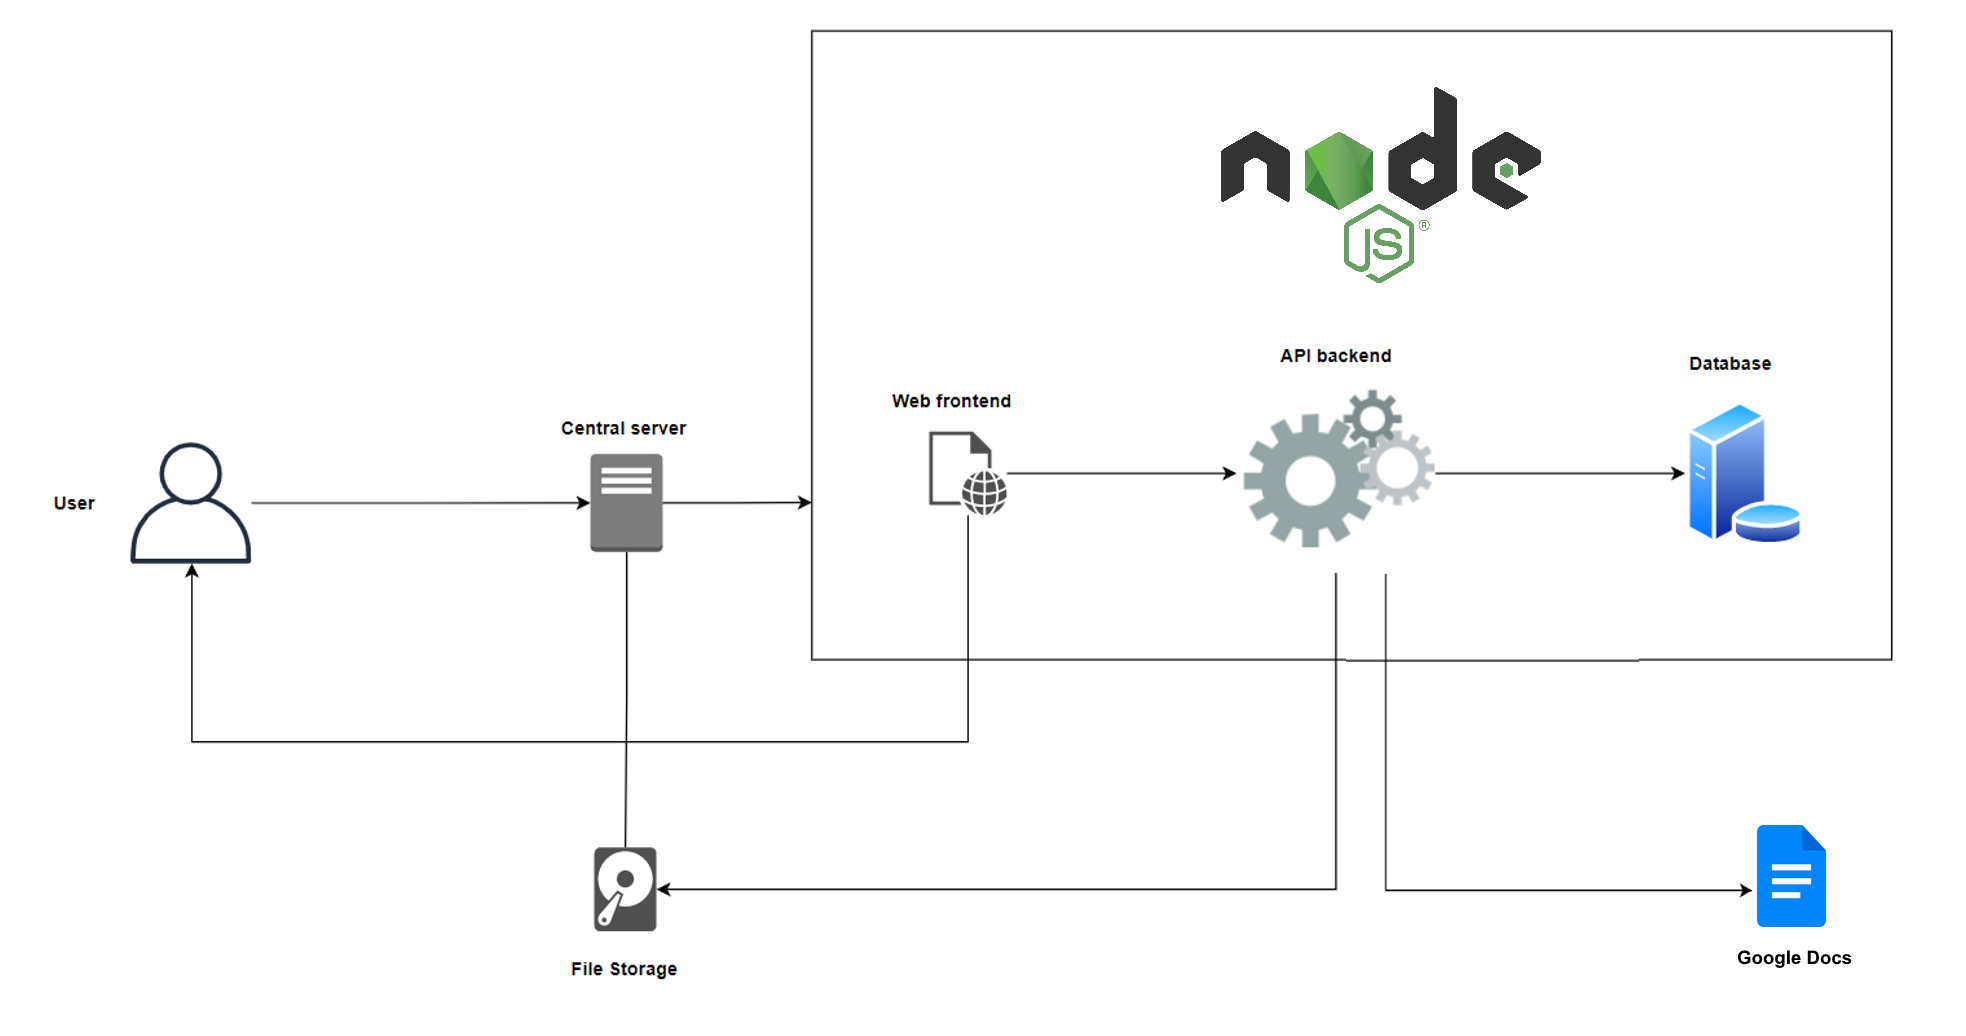
\includegraphics[scale=0.3]{images/software/architecture.png}
	\caption{A Zebrafish OS architektúrája, felülnézetből}
        \label{architecture}
\end{figure}

A Zebrafish operációs rendszer egy valós igényből született. Célunk az, hogy a konténereket egy szervergépen futtassuk egy modern operációs rendszeren, amely nem igényli ok nélkül függőségek sokaságát. Egy olyan biztonságos alapot szerettünk volna létrehozni, amelyet konténeres munkafolyamatok, például alkalmazások és weboldalak futtatására lehet használni.

A legtöbb operációs rendszer, például a Debian és az Ubuntu nem alkalmas erre a célra, mert túlságosan általánosak, és emiatt felesleges függőségeket hordoznak magukkal. Nem elég biztonságosak, és nem úgy tervezték őket, hogy konténeres környezetet futtassanak. Esettanulmány: az operációs rendszer egyetlen frissítése megtörheti az egész rendszer biztonságát. Egy Debian frissítés inspirálta a Zebrafish-t, mivel az egyik éles szerverem tűzfalai egyetlen csomagfrissítés után leálltak. Ez egy éles szerver esetében elfogadhatatlan, biztonsági résekhez vezethet. Ezért hoztuk létre a Zebrafish-t.

A Zebrafish fő ötlete, hogy egy immutable alapot biztosítson, amely képes konténerek futtatására. A Zebrafish egyetlen artifactként kerül kibocsátásra, amely bármely modern \texttt{x86\_64} vagy \texttt{ARM64} gépen elindítható. Az artifact két komponenst tartalmaz:
\begin{itemize}
    \item \textbf{Kernel} - A Linux kernel, amelyet a Zebrafish a rendszerindításhoz használ.
    \item \textbf{Gyökér fájlrendszer} - A Zebrafish gyökér fájlrendszere. Tartalmaz minden szükséges komponenst a Zebrafish OS futtatásához, beleértve a konténer futtattókörnyezetet, a rendszerdémonokat és a CLI eszközöket. Futás közben egy RAM-diskként él, biztosítva, hogy a rendszer mindig a memóriában cachelve legyen.
\end{itemize}

Minden frissítés során egy új artifact kerül kibocsátásra, amely tartalmazza a kernel és a root filesystem új verzióját. A Zebrafish frissítését egy manifest állomány segítségével végezzük, amely tartalmazza a kernel és a root filesystem hash értékét. A manifest állomány segítségével ellenőrizzük, hogy van-e szükség frissíŧésre, illetve hogy a letöltött frissítések helyesek-e. 

A Zebrafish operációs rendszer a következő nagyobb komponensekből áll:

\begin{enumerate}
        \item \textbf{Linux kernel} - A legújabb mainline kiadásra épül. Biztosítja a legújabb funkciók és frissítések elérhetőségét az optimális teljesítmény érdekében.
        \item \textbf{Gyökér fájlrendszer} - Tartalmazza az összes alapvető komponenst, amelyek szükségesek a Zebrafish operációs rendszer működéséhez:
        \begin{itemize}
                \item \textbf{Containerd} - Konténerek futtatására használt, könnyű és hatékony konténer futtatókörnyezet.
                \item \textbf{Zebrafish CLI (ocitool)} - Egy parancssori eszköz több-Compose-os projektek kezelésére.
                \item \textbf{Dropbear} - Egy pehelysúlyú SSH szerver, amelyet módosítottunk, hogy biztonsági okokból csak modern titkosítókészleteket engedélyezzen, és kötelezővé tettük a privát-kulcs alapú hitelesítést a fokozott biztonság érdekében.
                \item \textbf{Unbound} - DNS over HTTPS (DoH) rendszerdémon a biztonságos DNS domain-címek feloldása érdekében.
                \item \textbf{NTPd} - Biztosítja, hogy a rendszer órája szinkronban legyen a hálózati idővel a pontosság érdekében.
                \item \textbf{Crony} - Cron démon, amely időzített és ismétlődő feladatok kezelésére szolgál.
                \item \textbf{Zrepl (ZFS replication)} - Automatikus replikációt biztosít és időszakos biztonsági mentéseket végez az adatok biztonsága érdekében.
                \item \textbf{ACPId, udevd} - Hardver plug-and-play támogatást biztosít, lehetővé téve az eszközök zökkenőmentes kezelését.
                \item \textbf{syslogd} - Rendszer naplózási démon, amely a Zebrafish rendszer naplóit rögzíti.
        \end{itemize}
\end{enumerate}

Ezek közül a komponensek közül leginkább a konténerek futtatásához elengedhetetlen komponensekre fogunk koncentrálni, leginkább a \textit{containerd}-re és a Zebrafish CLI-ra (\texttt{ocitool}). A többi komponens elengedhetetlen a Zebrafish operációs rendszer futtatásához, de a jelenlegi téma szempontjából nagyrészt nem relevánsak. Érvelhetnénk azzal, hogy például az NTPd-t a rendszeróra szinkronizálására használjuk, ami ugyanaz az óra, amit minden konténer használ, de ez inkább pedáns lenne, mint hasznos.

\pagebreak

\section{A projekt mappaszerkezete}

\dirtree{%
.1 /.
.2 {/.github}.
.3 {workflows}.
.2 {/board}.
.3 {pc}.
.2 {/buildroot-packages}.
.3 {cni-plugins}.
.3 {containerd}.
.3 {\ldots}.
.2 {/buildroot-scripts}.
.3 {build.sh}.
.3 {prepare-artifacts.sh}.
.3 {\ldots}.
.2 {/configs}.
.3 {zebrafish\_aarch64\_defconfig}.
.3 {zebrafish\_x64\_defconfig}.
.2 {/images}.
.3 {zebrafish.svg}.
.2 {/package}.
.3 {dive}.
.3 {knockrs}.
.3 {\ldots}.
.2 {/patches}.
.3 {busybox}.
.3 {kbd}.
.2 {/rootfs-overlay}.
.3 {etc}.
.3 {lib}.
.3 {\ldots}.
.2 {.dockerignore}.
.2 {.gitignore}.
.2 {Config.in}.
.2 {INSTALL.md}.
.2 {README.md}.
.2 {users.txt}.
.2 {zebrafish-version.env}.
.2 {\ldots}.
}

\pagebreak

\begin{longtable}{|p{0.25\textwidth}|p{0.7\textwidth}|}
  \caption{Mappaszerkezet magyarázata}
  \hline
  \textbf{Mappa neve} & \textbf{Mappa tartalomjegyzéke} \\
  \hline
  .github & Tartalmazza a GitHub Actions munkafolyamatokat, amelyek automatizálják a Zebrafish operációs rendszer buildelését, tesztelését és releaselését minden commit után. \\
  \hline
  board & Tartalmazza a PC (x86\_64) architektúrához tartozó BIOS-specifikus konfigurációkat. \\
  \hline
  buildroot-packages & Egyedi Buildroot csomagokat tartalmaz, amelyeket a Zebrafish operációs rendszer felülírt custom változtatások, frissítések révén. Példa erre a containerd csomag, amelyet frissítettünk, hogy támogassa a ZFS snapshotter plugint. \\
  \hline
  buildroot-scripts & A Zebrafish operációs rendszer buildeléséhez, kitelepítéséhez szükséges shell scripteket tartalmazza. Példa erre a \texttt{build.sh} script, amely vezérli a Zebrafish rendszer teljes fordítási folyamatát, vagy például a \texttT{prepare-artifacts.sh} script, ami előkészíti a lebuildelt operációs rendszert a releasere  \\
  \hline
  configs & Tartalmazza a különböző architektúrákhoz (\texttt{ARM64}, \texttt{x86\_64}) tartozó Buildroot konfigurációs fájlokat, amelyek meghatározzák, hogy mely csomagok kerülnek be az operációs rendszerbe. \\
  \hline
  images & A projekthez tartozó grafikai elemeket tartalmazza: jelenleg a Zebrafish hivatalos logóját SVG formátumban. \\
  \hline
  package & Egyedi, Zebrafish-specifikus szoftver csomagokat tartalmaz, amelyek nem részei a standard Buildroot csomaggyűjteménynek. Erre példa például a \texttt{dive}, amely egy CLI program - segítségével meg lehet tekinteni a konténerimage-ek tartalmát debuggolás céljából, vagy a \texttt{knockrs}, amely a Zebrafish operációs rendszernek készített saját port knocking implementáció. \\
  \hline
  patches & Tartalmazza a meglévő upstream szoftverek módosításait (patch-eket), amelyek szükségesek a Zebrafish környezetben való megfelelő működés biztosításához. Jelenleg a \texttt{BusyBox} számára és a \textt{kbd} számára használunk patcheket, a \texttt{BusyBox} fordítási folyamatát javítja és a \texttt{kbd} csomagot optimalizálja. \\
  \hline
  rootfs-overlay & Tartalmazza a gyökér-fájlrendszer könyvtárstruktúráját. A végső root fájlrendszerbe bekerülnek ezek az állományok a Buildroot építési folyamat végén. \\
  \hline
\end{longtable}

\pagebreak

\section{Konténerek a containerd világában}

\figure{!h}
        \centering
        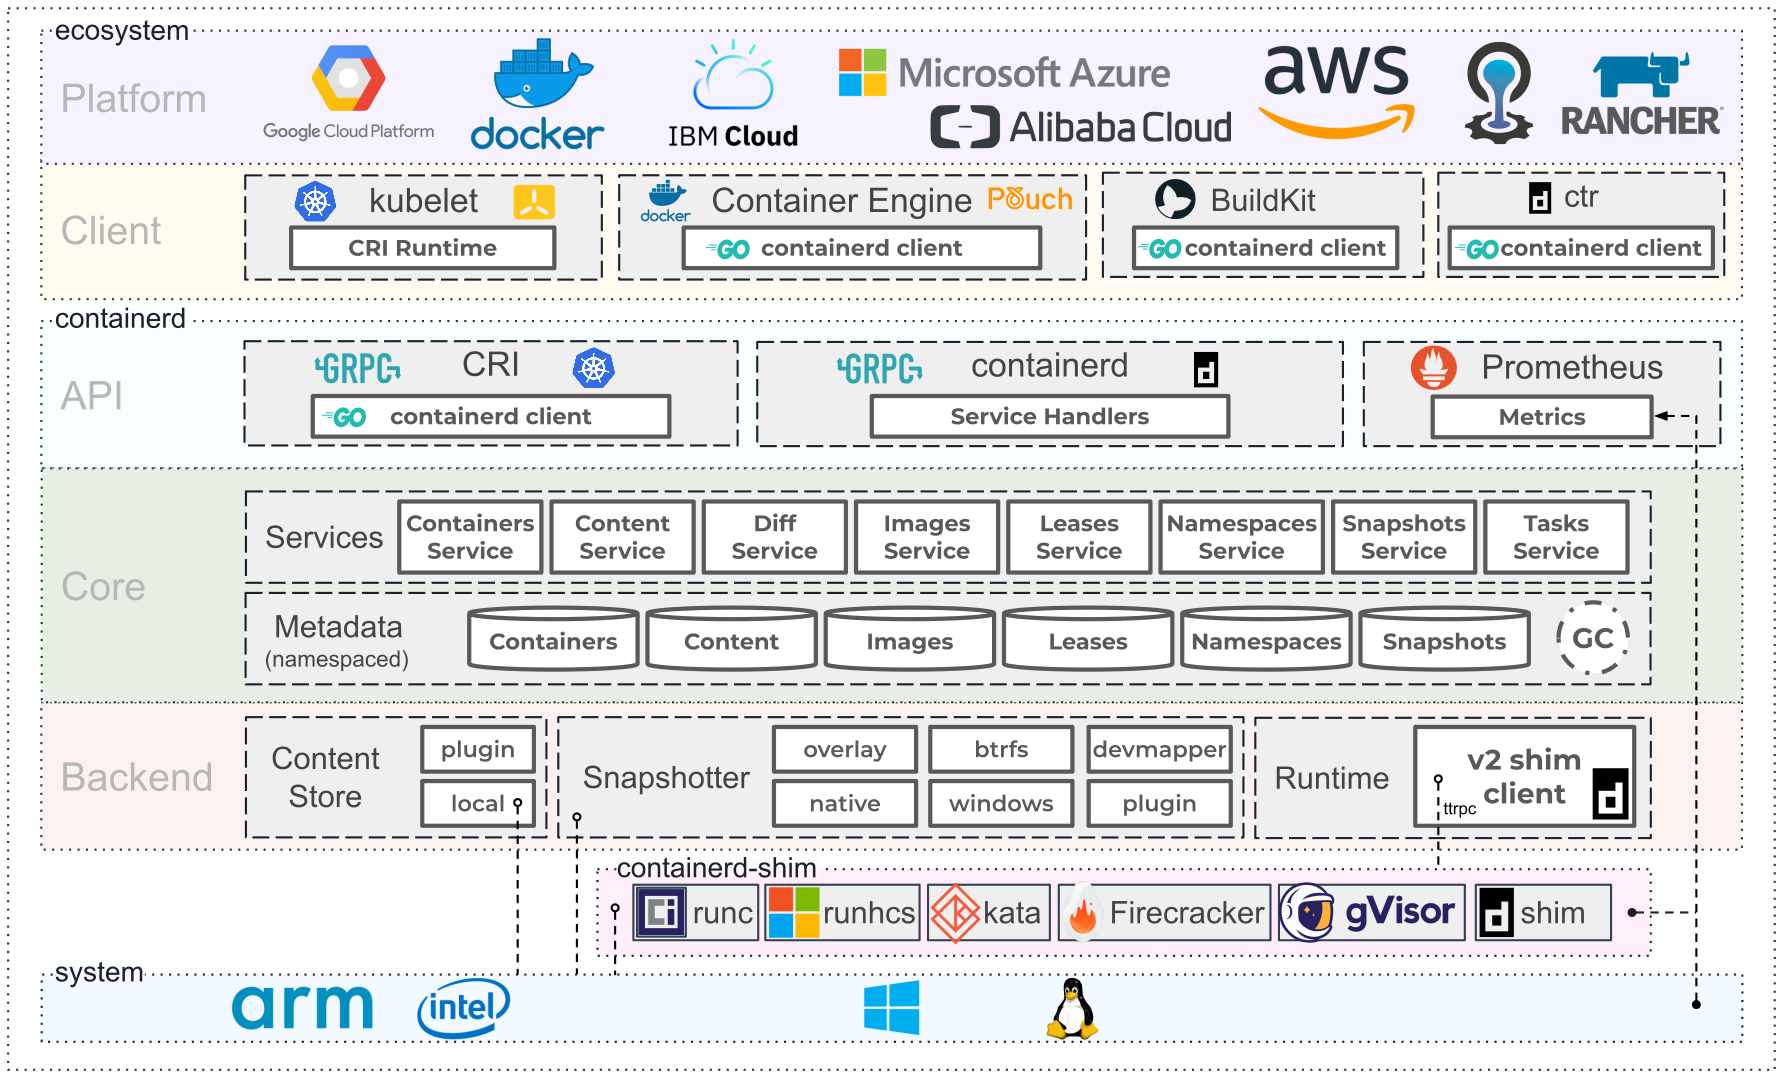
\includegraphics[scale=0.3]{images/software/containerd-architecture.png}
        \caption{A containerd architektúrája \cite{containerdhomepage}}
        \label{containerdarch}
\end{figure}

A konténerek forradalmasították a modern szoftverfejlesztést. De mi is történik valójában a háttérben, amikor egy konténert indítunk? A válasz megértéséhez betekintést kell nyernünk a \texttt{containerd} világába, amely a Docker és a Kubernetes alapjaként szolgált hosszú ideig.

A \texttt{containerd} egy magas szintű konténer futtatókörnyezet, amely az OpenContainers Runtime (OCR) specifikáció szerint működik. Ez a specifikáció határozza meg, hogyan kell a konténereket létrehozni, kezelni és futtatni a különböző platformokon. A containerd nem egyszerűen egy démonfolyamat, hanem egy teljes ökoszisztéma megtestesítője, amely gondoskodik a konténerek teljes életciklusáról, a letöltéstől a futtatásig.

Látni fogjuk, hogy a containerd valójában a konténer ökoszisztéma szíve, amely egységes felületet biztosít a konténerek kezeléséhez, azonban nem olyan magas szintű, mint egy konténer-orchestrációs platform. Nem biztosít például olyan funkciókat, mint a skálázás, a terheléselosztás vagy a szolgáltatásfelfedezés (\textit{service discovery}). Ezeket a funkciókat jellemzően a magasabb szintű orchestrációs platformok nyújtják, mint például a Kubernetes, vagy saját fejlesztésű platformokon a Docker Engine démon.

Az \ref{containerdarch}. ábrán látható a containerd architektúrája, és annak helye a szoftver-ökoszisztémában.

\section{Projektek összeállítása}

% example of docker-compose file, services, networks, etc.

\section{Miben különböznek a Multi-Compose projektek?}

% example of two interconnected compose files

\section{Image-ek frissítési folyamata (sequence diagram)}

\section{Hálózatok összeállítása hagyományos Dockerben}

\section{Hálózatok összeállítása Zebrafishben}

% example of network file : /etc/cni.d

\section{A konténerek közötti függőségek kiszámítása}

% hard dependencie
% soft dependencies

\section{Felhasználói use case-ek (use case diagram + table - pulling images)}

\section{Kliens-szerver architektúra}

\begin{figure}[!h]
	\centering
        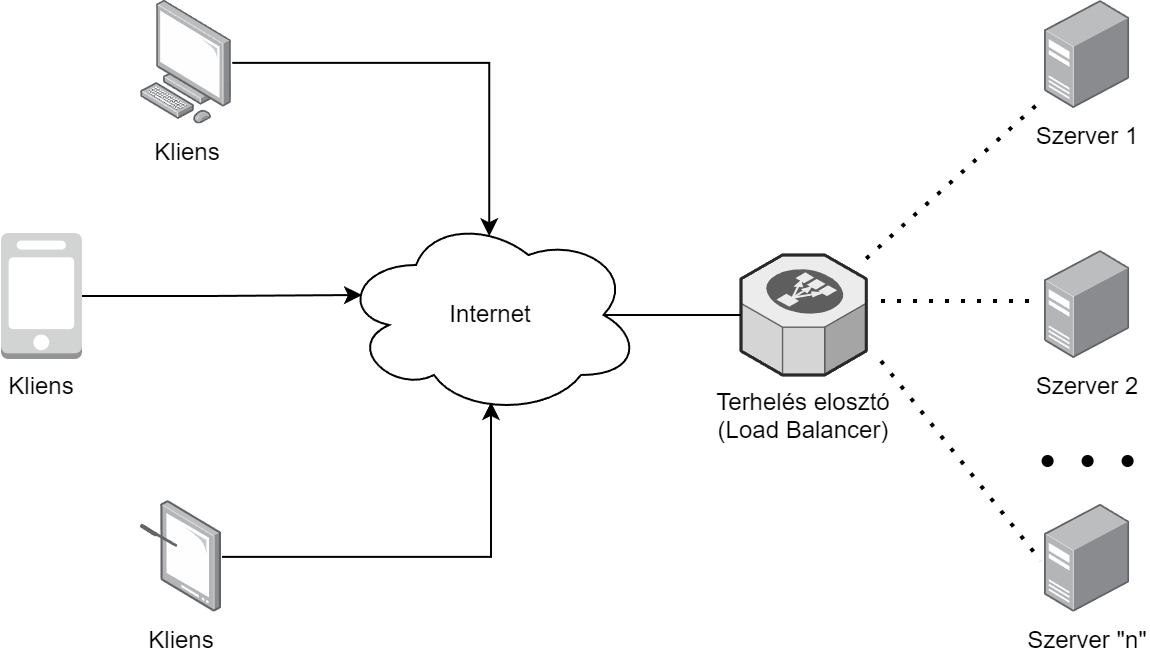
\includegraphics[scale=0.3]{images/software/client-server-arch.png}
	\caption{Tradicionális kliens-szerver architektúra}
        \label{csarch}
\end{figure}

A kliens-szerver architektúrában a felelősségek két kulcsfontosságú komponens - a kliens és a szerver - között oszlanak meg. A kliens-szerver architektúra magába foglalja a \textbf{kliens} fogalmát: egy felhasználóval szemben álló alkalmazást vagy felületet, amely kapcsolatként szolgál a felhasználó és a számítógép között, illetve a \textbf{szerver} fogalmát: egy biztonságos számítógépet, mely elvégzi az adatok feldolgozását.

A kliens és a szerver egy számítógépes hálózaton keresztül kommunikál egymással. A kliensek kéréseket küldenek a szerverek felé, a szerverek pedig a kért információk szolgáltatásával vagy a szükséges feladatok elvégzésével válaszolnak. Ez az architektúra lehetővé teszi a központi vezérlését az adott applikációnak, így alkalmas például webalapú rendszerek kiépítésére.

A Project Raccoon is kliens-szerver architektúrát alkalmaz, még \textit{serverless} környezetben is. A hagyományos telepítések során a Project Raccoon egy központi szerverre van telepítve, amely gondoskodik az API backendről, a frontendről és opcionálisan az adatbázisról és a fájltárolásról is. A szerver nélküli \textit{serverless} telepítések esetén sem beszélünk teljesen szerver \textit{nélküli} architekturáról: a szerver automatikusan elindul, amikor a kliensek információt kérnek a szolgáltatástól.

A \ref{csarch} ábrán látható egy tradicionális kliens-szerver architektúra. A kliensek kéréseket tesznek a szolgáltatás felé. Ezek a kérések átmennek az interneten, amely a kérésüket a terhelés elosztónkhoz (\textit{load balancer}-hez) irányítja, függetlenül attól, hogy a kliensek földrajzilag hol helyezkednek el. 

A \textit{load balancer} feladata, hogy kiossza a beérkező kéréseket a rendelkezésre álló szerverek között. Ez lehetővé teszi a rendszer vertikális skálázását, és megelőzi, hogy bármelyik szerver túlterheltté váljon. A \textit{load balancer} a kérések útbaigazításához több stratégiát vethet be. \cite{loadbalancing} Ezek közül megemlítenék egy párat:

\begin{itemize}
  \item \textbf{Körkörös teherelosztás (\textit{Round-robin balancing})}: Egy egyszerű elvet követ. Körkörösen váltogatja a kiszolgáló szervert a rendelkezésre álló kiszolgálók listájából. Minden új kérést szekvenciálisan a listán következő szerverhez rendelünk, biztosítva ezzel, hogy a munkaterhelés egyenletesen oszlik el az összes rendelkezésre álló erőforrás között. A körkörös terheléselosztás megakadályozza egyetlen kiszolgáló szerver túlterhelését, miközben maximalizálja a rendszer általános teljesítményét és átbocsátóképességét. Ez a megközelítés könnyen megvalósítható, skálázható, és egyszerű módot biztosít a nagy mennyiségű kérések kiegyensúlyozott kezelésére. \cite{loadbalancing}
  \item \textbf{Legkisebb kapcsolaton alapuló tehereloszlás (\textit{Least-connection load balancing})}: Célja, hogy a bejövő kéréseket több az aktuális terhelési szint alapján ossza el. Ez a technika arra törekszik, hogy minimalizálja az egyes kiszolgáló szerverek által kezelt kapcsolatok számát. \cite{loadbalancing} Biztosítja, hogy a munkaterhelés egyenletesen osztódjon el az összes rendelkezésre álló erőforrás között. Amikor új kérés érkezik, a \textit{load balancer} dinamikusan kiválasztja azt a szervert, amelyik a legkevesebb aktív kapcsolattal rendelkezik, és a kérést ehhez rendeli hozzá. Ez minimalizálja a szerver túlterhelésének kockázatát. Ez a megközelítés különösen hatékony olyan esetekben, ahol a szerverek kapcsolatterhelése jelentősen változhat.
  \item \textbf{IP-címen alapú tehereloszlás (\textit{IP hash load balancing})}: A bejövő kérések forrásának IP-címe alapján kiszámít egy hash-értéket, és hozzárendeli azt az egyik elérhető kiszolgálóhoz. A hozzárendelés konzisztens marad az azonos IP-címről érkező későbbi kérések esetében, így biztosítva, hogy egy adott kliens minden kérése ugyanarra a kiszolgálóra irányuljon. Azáltal, hogy a IP-címet használja a terheléselosztás kulcsaként,  biztosítja, hogy a felhasználók munkamenetének késleltetése azonos marad. \cite{loadbalancingtech} Ez különösen létfontosságú a valós idejű alkalmazásoknál, ahol fontos, hogy a késleltetés mértéke egyenletes maradjon. A \textit{Project Raccoon} is tartalmaz valós idejű komponenseket - nevezetesen valós idejű csevegést biztosít az eladó és a vevő között a szerződéstárgyalások során.
\end{itemize}

Nem mindig szükséges terheléselosztó használata, de erősen ajánlott, ha előre látható, hogy nagyon sok felhasználó fogja használni a szolgáltatásunkat. Ha nincs terheléselosztó, akkor a kliensek automatikusan egy központi kiszolgáló szerverhez (\textit{central server}) csatlakoznak. Ebben az esetben a szerverek kiválasztásában nem játszik szerepet terheléselosztó algoritmus, mivel mindig csak egy szerver áll rendelkezésre. Ez azonban különösen veszélyes, mert ha a központi kiszolgáló szerver összeomlik vagy más módon elérhetetlenné válik, nem marad egyetlen kiszolgáló sem, amely a beérkező kéréseket kezelné.

A terheléselosztás különösen fontos, hogy a szolgáltatás leállási ideje (\textit{downtime}) minimális legyen. Ezért a \textit{Project} Raccoon úgy van felépítve, hogy lehetővé tegye a vertikális skálázás használatát. Ez nem feltétlenül szükséges - a \textit{Project Raccoon}-t továbbra is lehet futtatni az összes architekturális többletköltség nélkül, például több adatbázis telepítése, terheléselosztók és több szerver konfigurálása nélkül.

\begin{figure}[!h]
	\centering
        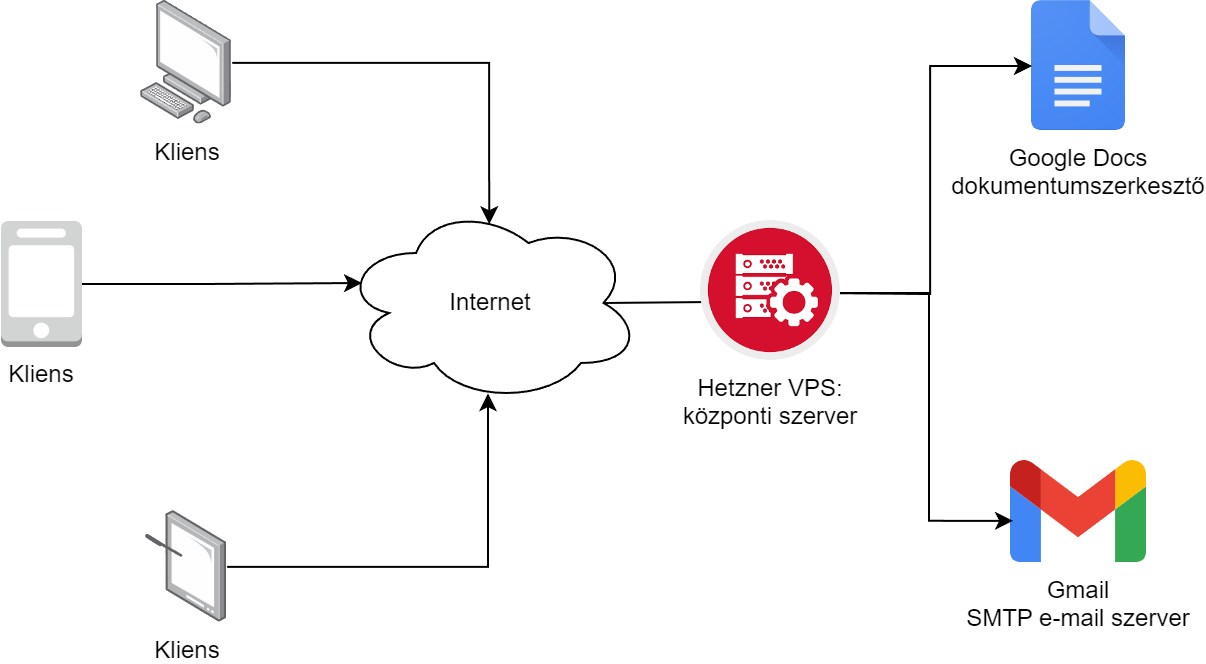
\includegraphics[scale=0.37]{images/software/simplest-architecture.png}
	\caption{A \textit{Project Raccoon} legegyszerűbb kliens-szerver kivitelezése}
        \label{simplestarch}
\end{figure}

A \ref{simplestarch} ábrán látható a \textit{Project Raccoon} legegyszerűbb kitelepítése. Maga a Project Raccoon által szolgáltatott web frontend, API backend, az adatbázisok és a fájltárolás egy Hetzner virtuális számítógép által vannak szolgáltatva. Ebben az esetben a terhelés nincs kiegyenlítve. Ha a Hetzner VPS meghibásodik vagy leáll, a szolgáltatás teljesen elérhetetlenné válik. Megengedhetjük magunknak, hogy az adatbázist és a fájltárolót ezen az egy szerveren hosztoljuk, mert csak ennek az egy szervernek kell hozzáférnie ezekhez.

A \ref{simpleprocon} táblázatban levezetjük ennek a megoldásnak az előnyeit és hátrányait. Mivel ennek a megközelítésnek nagyon erős hátrányai vannak, ajánlott egy bonyolultabb, de nagyobb teljesítményű telepítési architektúrát választani.

\pagebreak

\begin{table}
\begin{tabularx}{\linewidth}{>{\parskip1ex}X@{\kern4\tabcolsep}>{\parskip1ex}X}
\toprule
\hfil\bfseries Előnyök
&
\hfil\bfseries Hátrányok
\\\cmidrule(r{3\tabcolsep}){1-1}\cmidrule(l{-\tabcolsep}){2-2}

Nincs korlátja annak, hogy mit tehetünk a szerveroldalon.\par
A szerver mindig gyorsan válaszol, hiszen nem szükséges külső szolgáltatásokra várakozni.\par
Relatív kevés anyagi erőforrást igényel.\par
Egyszerű felépítése révén könnyen telepíthető és futtatható is.\par
A Docker használatával bármilyen architektúrájú processzorra kitelepíthető, például ARM szerverekre is. \cite{dockerarm}\par

&

Szükséges egy szerver kibérlése, bekonfigurálása és folyamatos üzemeltetése.\par
Nem skálázható vertikálisan - nem tud nagy mennyiségű felhasználót kiszolgálni.\par
Vízszintes skálázás esetén a szerver erőforrásainak kibővítése rendkívül költséges lehet.\par
A telepítés gyakran unalmasabb, és Linux szerver ismereteket igényel.\par
\\\bottomrule
\end{tabularx}
\caption{A legegyszerűbb kivitelezés előnyei és hátrányai}
\label{simpleprocon}
\end{table}

\begin{figure}[!h]
	\centering
        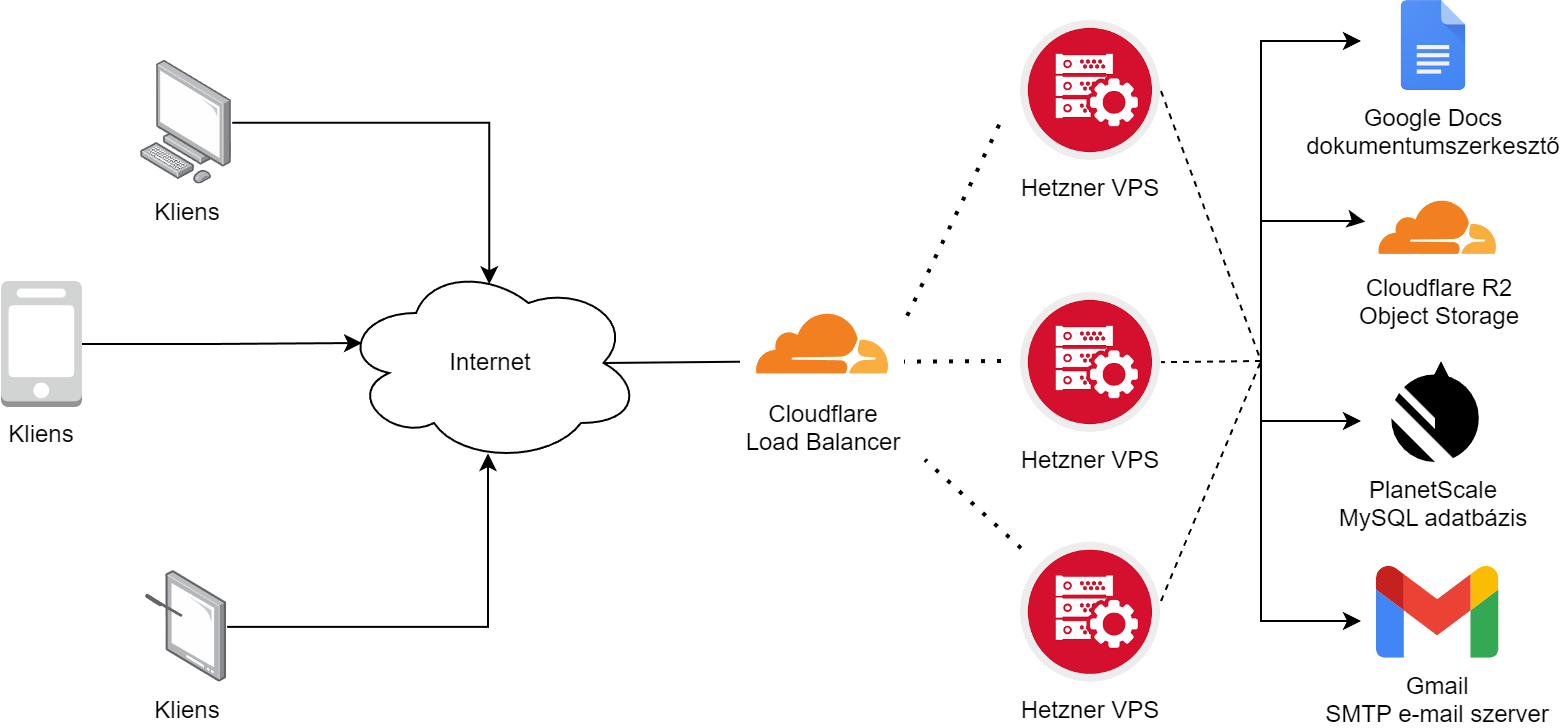
\includegraphics[scale=0.28]{images/software/detailed-arch.png}
	\caption{A \textit{Project Raccoon} részletesebben kidolgozott telepítésének kivitelezése}
        \label{detailedarch}
\end{figure}

A \ref{detailedarch} ábrán látható a \textit{Project Raccoon} részletesebben kidolgozott telepítésének felvázolása. Ebben az esetben is marad a hagyományos szerver-kliens architektúra, hiszen a centralizált szervert felváltja három, egymástól független Hetzner virtuális gép.

Mivel már három különböző szerverről beszélünk, ezért át kell gondoljuk a szerverek hatáskörét. Az előző megvalósításban az adatbázis, illetve a fájlok tárolása egyetlen egy szerveren történt, nem volt szükség külső szolgáltatás használatára. Ebben az esetben viszont szigorúan el kell különítsük a szerverektől az adatokat tárolását. Hogyha az adatokat ugyanazon a szerveren tároljuk, akkor az az adott szerver könnyen túlterheltté váik. Hogyha az adatokat külön-külön minden szerveren tároljuk, akkor redundáns adattárolás történik, sőt, szinkronizálnunk kell az adatokat az összes szerver között, ami egyáltalán nem egyszerű dolog.

Két új szolgáltatást vezetünk be: egy automatikusan önskálázó adatbázis-szolgáltatót, a \textit{PlanetScale}-t illetve a Cloudflare R2 \textit{Object Storage}-t. A \textit{PlanetScale} feladata, hogy a három szerverünk felé szolgáltasson egy olyan adatbázist, amely automatikusan skálázza magát, és bármely időpillanatban elérhető a szerverek számára. A relációs adatbázisunk adatait ebben a rendszerben tárolhatjuk. A három szerver ezentúl nem tárolja saját magában az adatbázis adatait. Hasonlóképpen, a Cloudflare R2 \textit{Object Storage} átveszi a fájltárolás feladatait a Hetzner VPS-től. A Cloudflare R2 centralizált tárolóhelyet biztosít a \textit{Project Raccoon}-nak, lehetőséget adva a rendszernek, hogy itt tárolja a végleges szerződéseket, esetlegesen feltöltött mellékleteket, illetve a felhasználók profilképeit.

A \ref{detailedprocon} táblázatban levezetjük e megoldás előnyeit és hátrányait. Mivel ez a megoldás kevesebb hátránnyal rendelkezik, már alkalmazható huzamosabb ideig, több felhasználó kiszolgálására is.

\begin{table}
\begin{tabularx}{\linewidth}{>{\parskip1ex}X@{\kern4\tabcolsep}>{\parskip1ex}X}
\toprule
\hfil\bfseries Előnyök
&
\hfil\bfseries Hátrányok
\\\cmidrule(r{3\tabcolsep}){1-1}\cmidrule(l{-\tabcolsep}){2-2}

Vertikálisan skálázható, új szerverek hozzáadásával a rendszerben.\par
A szervereket nem terhelik túl a felhasználók kérései.
A Docker használatával egyszerűsíthető a szerverek kitelepítése.\par
Ha megsemmisülnek a szerverek egy hiba során, az adatok megmaradnak a Cloudflare object storage-ban és a PlanetScale adatbázisában.\par
A Cloudflare és a PlanetScale automatikus biztonsági mentéseket végeznek az adatokról.\par

&

Még mindig szükséges a szerverek kibérlése. Mivel több szervert bérlünk, ezért több pénzbe kerül a rendszer futtatása.\par
Nem skálázható vertikálisan - nem tud nagy mennyiségű felhasználót kiszolgálni.\par
Ha nincsen túl sok felhasználónk, nincs értelme egy ennyire komplex kitelepítési architekturát érvénybe léptetni.\par
A telepítés még mindig Linux szerver ismereteket igényel.\par
A PlanetScale adatbázisa kicsit különbözik a megszokott MySQL adatbázisoktól, így fennáll a \textit{vendor lock-in} veszélye. (A vendor lock-in olyan helyzetet jelent, amikor erősen függünk egy adott szolgáltatástól, ami megnehezíti vagy költségessé teszi az alternatív szolgáltatásokra való váltást.)
\\\bottomrule
\end{tabularx}
\caption{A kidolgozott kivitelezés előnyei és hátrányai}
\label{detailedprocon}
\end{table}

\section{Serverless architektúra}

\begin{figure}[!h]
	\centering
        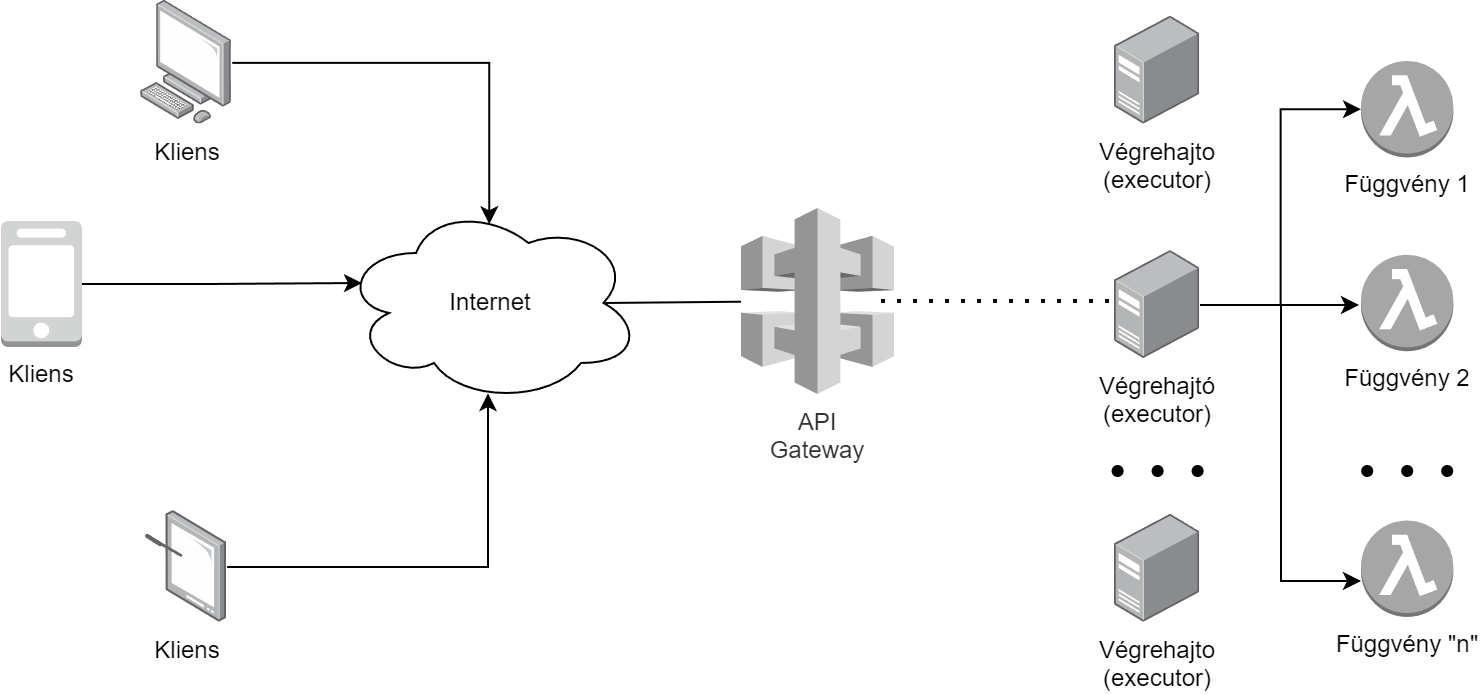
\includegraphics[scale=0.3]{images/software/serverless.png}
	\caption{Kliens-szerver architektúra megvalósítása serverless technológiával}
        \label{serverless}
\end{figure}

A \textit{serverless} architektúra egy felhőalapú modellre utal, ahol az infrastruktúra és a szerver menedzsment feladatai el vannak vonatkoztatva a fejlesztőktől, így azok kizárólag a kód írására és telepítésére koncentrálhatnak. Ez a megközelítés kiküszöböli a szerverek rendelkezésre bocsátásának, konfigurációjának és kezelésének szükségességét, mivel a felhőszolgáltató dinamikusan kezeli a kód végrehajtásához szükséges erőforrásokat. Mivel a \textit{Project Raccoon} alkalmazást a Next.js keretrendszerének kontextusában építettük fel, az alkalmazás teljes mértékben kitelepíthető \textit{serverless} technológiákkal is. A \textit{serverless} technológiák segítségével a \textit{Project Raccoon} kitelepítése egyszerűbbé és skálázhatóbbá válik.

A szerver nélküli kitelepítés stratégiájával a weboldalunk minden egyes elérhetőségét egy külön függvényként kitelepítjük a serverless felhőbe. Ezek a függvények mindig élnek a felhőben, viszont csak akkor futnak, mikor a felhasználók kérik. Mikor egy kérés érkezik egy felhasználó számáról,  a kérés legelőször egy API Gateway-hez kerül. Az API Gateway megkeresi a felhőben lementett függvény lokációját, ahol tárolva van a függvény. Ezután megnézi, hogyha már van olyan szerver a felhőben, amely jelenleg futtatja az adott függvényt. Ha van, a kérést ahhoz a szerverhez továbbítja, ahol a kért függvény fut. Ha nincs, akkor keres egy olyan szervert, amely nincs túlságosan lefoglalva kérésekkel. A kapott szerver letölti a felhőből a függvény forráskódját, és elkezdi futtatni. Ezt nevezik hidegindításnak (angolul: \textit{cold boot}). Sajnos ez enyhe késleltetést eredményez az olyan alkalmazások esetében, amelyeket egy ideje nem használt egyetlen felhasználó sem. A hideginditás után, ha az alkalmazást nem használja huzamosabb ideig egyetlen felhasználó sem, a függvény lekapcsolódik és új kérés esetén újra szükségessé válik egy új szerver keresése és a függvény újratelepítése (mégegy hidegindítás szükséges). \cite{serverlessbib}

A Project Raccoon esetében a \textit{serverless} technológiákkal való kitelepítést a Vercel platform használatával ajánljuk. Mivel a Next.js keretrendszert a Vercel készítette, ezért nyílvánvaló, hogy a Next.js teljes mértékben fel van szerelve a \textit{serverless} technológiák támogatására. A \textit{serverless} telepítés során ugyancsak szükséges az alkalmazás összekötése a Google Docs, Cloudflare R2, PlanetScale és Gmail rendszerekkel. A Cloudflare Load Balancer szerepét lecseréli a Vercel API gatewayje, amely a Vercel hálózatában automatikusan kiosztja a szerver nélküli függvények a kiszolgáló szerverek között. Nincs szükség saját szerver futtatására, karbantartására.

A \ref{serverlessprocon} táblázatban a \textit{serverless} megközelítés előnyeit és hátrányait tárgyaljuk. Ez a megközelítés olyan esetben megfelelő, amikor vagy alig felhasználó, és nincs igazi oka egy teljes szerver felállításának, vagy akkor, amikor olyan sok felhasználó van, hogy nagyon nehéz lenne egy egész szervercsoportot (\textit{server cluster}-t) kezelni.

\begin{table}
\begin{tabularx}{\linewidth}{>{\parskip1ex}X@{\kern4\tabcolsep}>{\parskip1ex}X}
\toprule
\hfil\bfseries Előnyök
&
\hfil\bfseries Hátrányok
\\\cmidrule(r{3\tabcolsep}){1-1}\cmidrule(l{-\tabcolsep}){2-2}

Könnyű telepítés és skálázhatóság\par
Kevesebb időtöltés szerverek beállításával\par
Nem szükségesek a Linux szerver adminisztráció lépéseinek ismerete.\par
Nincs szükség külön szerverre - minden a szerver nélküli funkciókon fut a felhőben.\par
Kevés felhasználó esetén sokkal olcsóbb a szolgáltatás serverless futtatása, mint a szerver bérlése.\par

&

A serverless szolgáltató által előírt összes korlátozás érvényesek.\par
Egy esetleges DDoS (\textit{Distributed Denial of Service}) támadás során a szolgáltatás működtetésének költségei az egekbe szökhetnek, nagy anyagi károkat okozva.\par
A hidegindítások nagyon lassúvá teszik a kapcsolat létesítését a szolgáltatással, ha hosszabb ideig nem használják.\par

\\\bottomrule
\end{tabularx}
\caption{A serverless kivitelezés előnyei és hátrányai}
\label{serverlessprocon}
\end{table}

\pagebreak

\section{MVC - Modell-Nézet-Vezérlő}

A \textit{Project Raccoon} keretén belül az MVC szoftver architektúrális mintát használjuk. Az \textbf{MVC} - Modell-Nézet-Vezérlő minta megengedi nekünk, hogy a kódbázisunkat moduláris modulokból építsük fel.

A modell képviseli az alkalmazás adatait és üzleti logikáját, és kezeli az adatbázisokkal és külső szolgáltatásokkal való adatinterakciókat. A nézet (\textit{view}) kezeli az adatok megjelenítését a felhasználók számára, felhasználói felületét jelképezve a szoftvernek. A modell és a nézet közötti hídként működő Vezérlő kezeli a felhasználók kéréseit, dolgozza fel az adatokat, és ennek megfelelően frissíti a modellt és olykor a nézetet. A felelősségek egyértelmű szétválasztása ily módon megkönnyíti a kód karbantartását.

\subsection{Modellek}

A \textit{Project Raccoon} az adatok modellezésére a TypeORM keretrendszert használja. A TypeORM keretén belül a TypeScript-el megírt osztályok automatikusan leképezhetőek relációs és nem-relációs adatbázisokra is egyaránt. A relációs adatbázis sémák metaadatait, mint több más hasonló keretrendszerben is, a modellekben megadhatjuk dekorátorok segítségével. Minden modellünk két részből áll:

\begin{enumerate}
  \item egy \textbf{interfészből}, amely meghatározza az entitás adattaigjait egy általános, nem TypeORM-specifikus módon - lásd \ref{code:modelinterface} kódrészlet;
  \item illetve egy \textbf{TypeORM entitásból}, amely implementálja az interfészt, TypeORM-specifikus és metaadatokat is tartalmaz dekorátorok formájában - lásd \ref{code:modelentity} kódrészlet.
\end{enumerate}

\begin{lstlisting}[caption={ Egy modell interfészének megvalósítása }, captionpos=b, language = TS, label={code:modelinterface}]
export interface IItem {
  id?: number;
  createdAt?: Date;
  updatedAt?: Date;
  friendlyName?: string;
  slug?: string;
  description?: string;
  options?: IItemOption[];
}
\end{lstlisting}

\pagebreak

\begin{lstlisting}[caption={ Egy modell entitásának megvalósítása }, captionpos=b, language = TS, label={code:modelentity}]
@Entity()
export class Item implements IItem {
  @PrimaryGeneratedColumn()
  id: number;

  @CreateDateColumn()
  createdAt: Date;

  @UpdateDateColumn()
  updatedAt: Date;

  @DeleteDateColumn()
  deletedAt?: Date;

  @Column()
  friendlyName: string;

  @Column({ unique: true })
  slug: string;

  @Column()
  description: string;

  @OneToMany(() => ItemOption, (itemOption) => itemOption.item)
  options: Partial<ItemOption[]>;
}
\end{lstlisting}

\subsection{Nézetek}

A \textit{Project Raccoon}-ban a nézetek React komponenseknek felelnek meg. Hosszú csata folyik a React programozók között. Néhányan a régi, osztályalapú megközelítést részesítik előnyben a React felhasználói felület komponensek létrehozásakor, míg mások az újabb, funkcionális megközelítést szeretik jobban. Mi a funkcionális komponensek mellett döntöttünk. Ez azt jelenti, hogy ahelyett, hogy minden React nézetet egy osztályként hozunk létre, helyette minden nézet egy-egy függvénynek írunk meg. Ezért nem is tudunk szolgáltatni hagyományos osztálydiagrammal.

Az osztály-alapú nézetek és a funkcionális nézet között a legnagyobb különbség, hogy míg az osztály-alapú nézetekben explicit módon meg kell határozni az állapotváltozókat és minden más adatforrást, a funkcionális komponensek esetén használható a függőség befecskendezés fogalma (angolul: \textit{dependency injection}), lásd: \ref{code:depinj}. kódrészlet.

\begin{lstlisting}[caption={ A felhasználó objektum befecskendezése egy React komponensbe }, captionpos=b, language = TS, label={code:depinj}]
const LoginForm = () => {
  const [user, setUser] = useCurrentUser();

  if (user) {
    return <p>You are already logged in as {user.username}!</p>;
  }

  return (
    <form>
      ...
    </form>
  );
}
\end{lstlisting}

\subsection{Vezérlők}

A \textit{Project Raccoon} rendszeren belül csupán a vezerlők képesek módosítani közvetlenül a modelleken. A vezerlők a \textit{controllers} mappában élnek, és entitás szerint csoportosítva vannak. Minden egyes vezérlő minden egyes függvényére hivatkozik egy API route a \textit{pages/api} mappából.

A \textit{next-bar} csomag használatával a \textit{pages/api} mappában meghatározhatunk API útvonalakat (\ref{code:apiroute}. kódrészlet). Ezek az API útvonalak a HTTP metódus típusa alapján kerülnek kiválasztásra, mint például POST, GET, DELETE stb.

\pagebreak

\begin{lstlisting}[caption={ Példa implementáció egy API útvonalra, mely egy vezérlőre csatlakozik }, captionpos=b, language = TS, label={code:apiroute}]
import bar from 'next-bar';
import { ensureAdministrator } from '@/middleware/auth';
import * as contractOptionsController from '@/controllers/contract-options/contractOptionsController';

export default bar({
  post: ensureAdministrator(contractOptionsController.newContractOption),
  get: ensureAdministrator(contractOptionsController.listContractOptions),
});
\end{lstlisting}

Ez esetben a vezérlő a \textit{controllers/contract-options/contractOptionsController.ts} állományban él. Két függvényt tartalmaz. Az egyik függvény egy POST hívásra létrehoz egy új szerződés sablon opciót, a másik függvény pedig egy GET hívásra kilistázza az összes szerzdős sablon opciót. A vezérlő feladata, hogy kiolvassa a HTTP kérésekből a szükséges információkat, és hogy hajtsa végre a kért műveletet. Abban az esetben, hogyha olyan megszorítások vannak egy API útvonalra, amelyek nem teljesülnek, a kérés nem hajtódik végre. A \ref{code:apiroute}. kódrészletben például mindkét funkcionalitás csak akkor érhető el, hogyha a felhasználó adminisztrátor felhasználó.

Fontos megemlíteni, hogy a fő vezérlő fájlokban csupán a HTTP kérések feldolgozása hajtódik végre. Minden üzleti logikát, aszerint, hogy mit hajt végre, külön fájlban implementáltunk ugyanabban a modulban. Ez esetben például a ``\textit{newContractOption}'' függvényhez tartozik egy \textit{controllers/contract-options/newContract.ts} állomány is, amely végrehajta a szószerinti üzleti logikát.

\section{Szolgáltatási réteg}

A felhasználói felület a HTTP-kéréseket nem közvetlenül a felhasználói felületből indítja, hanem a szolgáltatási rétegnek delegálja. A szolgáltatási réteg a \textit{Project Raccoon} azon modulja, amely a fejlesztőtől elabsztraktizálja a HTTP kérések logikáját, és az entitásokhoz tartozó szolgáltatásokban gondolkozik. Amikor a felhasználói felületnek egy műveletet kell végrehajtania, vagy adatokat kell kérnie az API-tól, az adott entitásért felelős szolgáltatással lép kapcsolatba, ahelyett, hogy magára HTTP-kérést intézne. Ez nagyon megkönnyíti egy stabil API létrehozását, amelyet nagyon nehéz helytelenül használni, mivel az összes API-specifikus kommunikációt különálló modulokba szét lehet választani és külön-külön tesztelni lehet.

\section{Szerződéssablonok létrehozása}

\begin{figure}[!h]
	\centering
        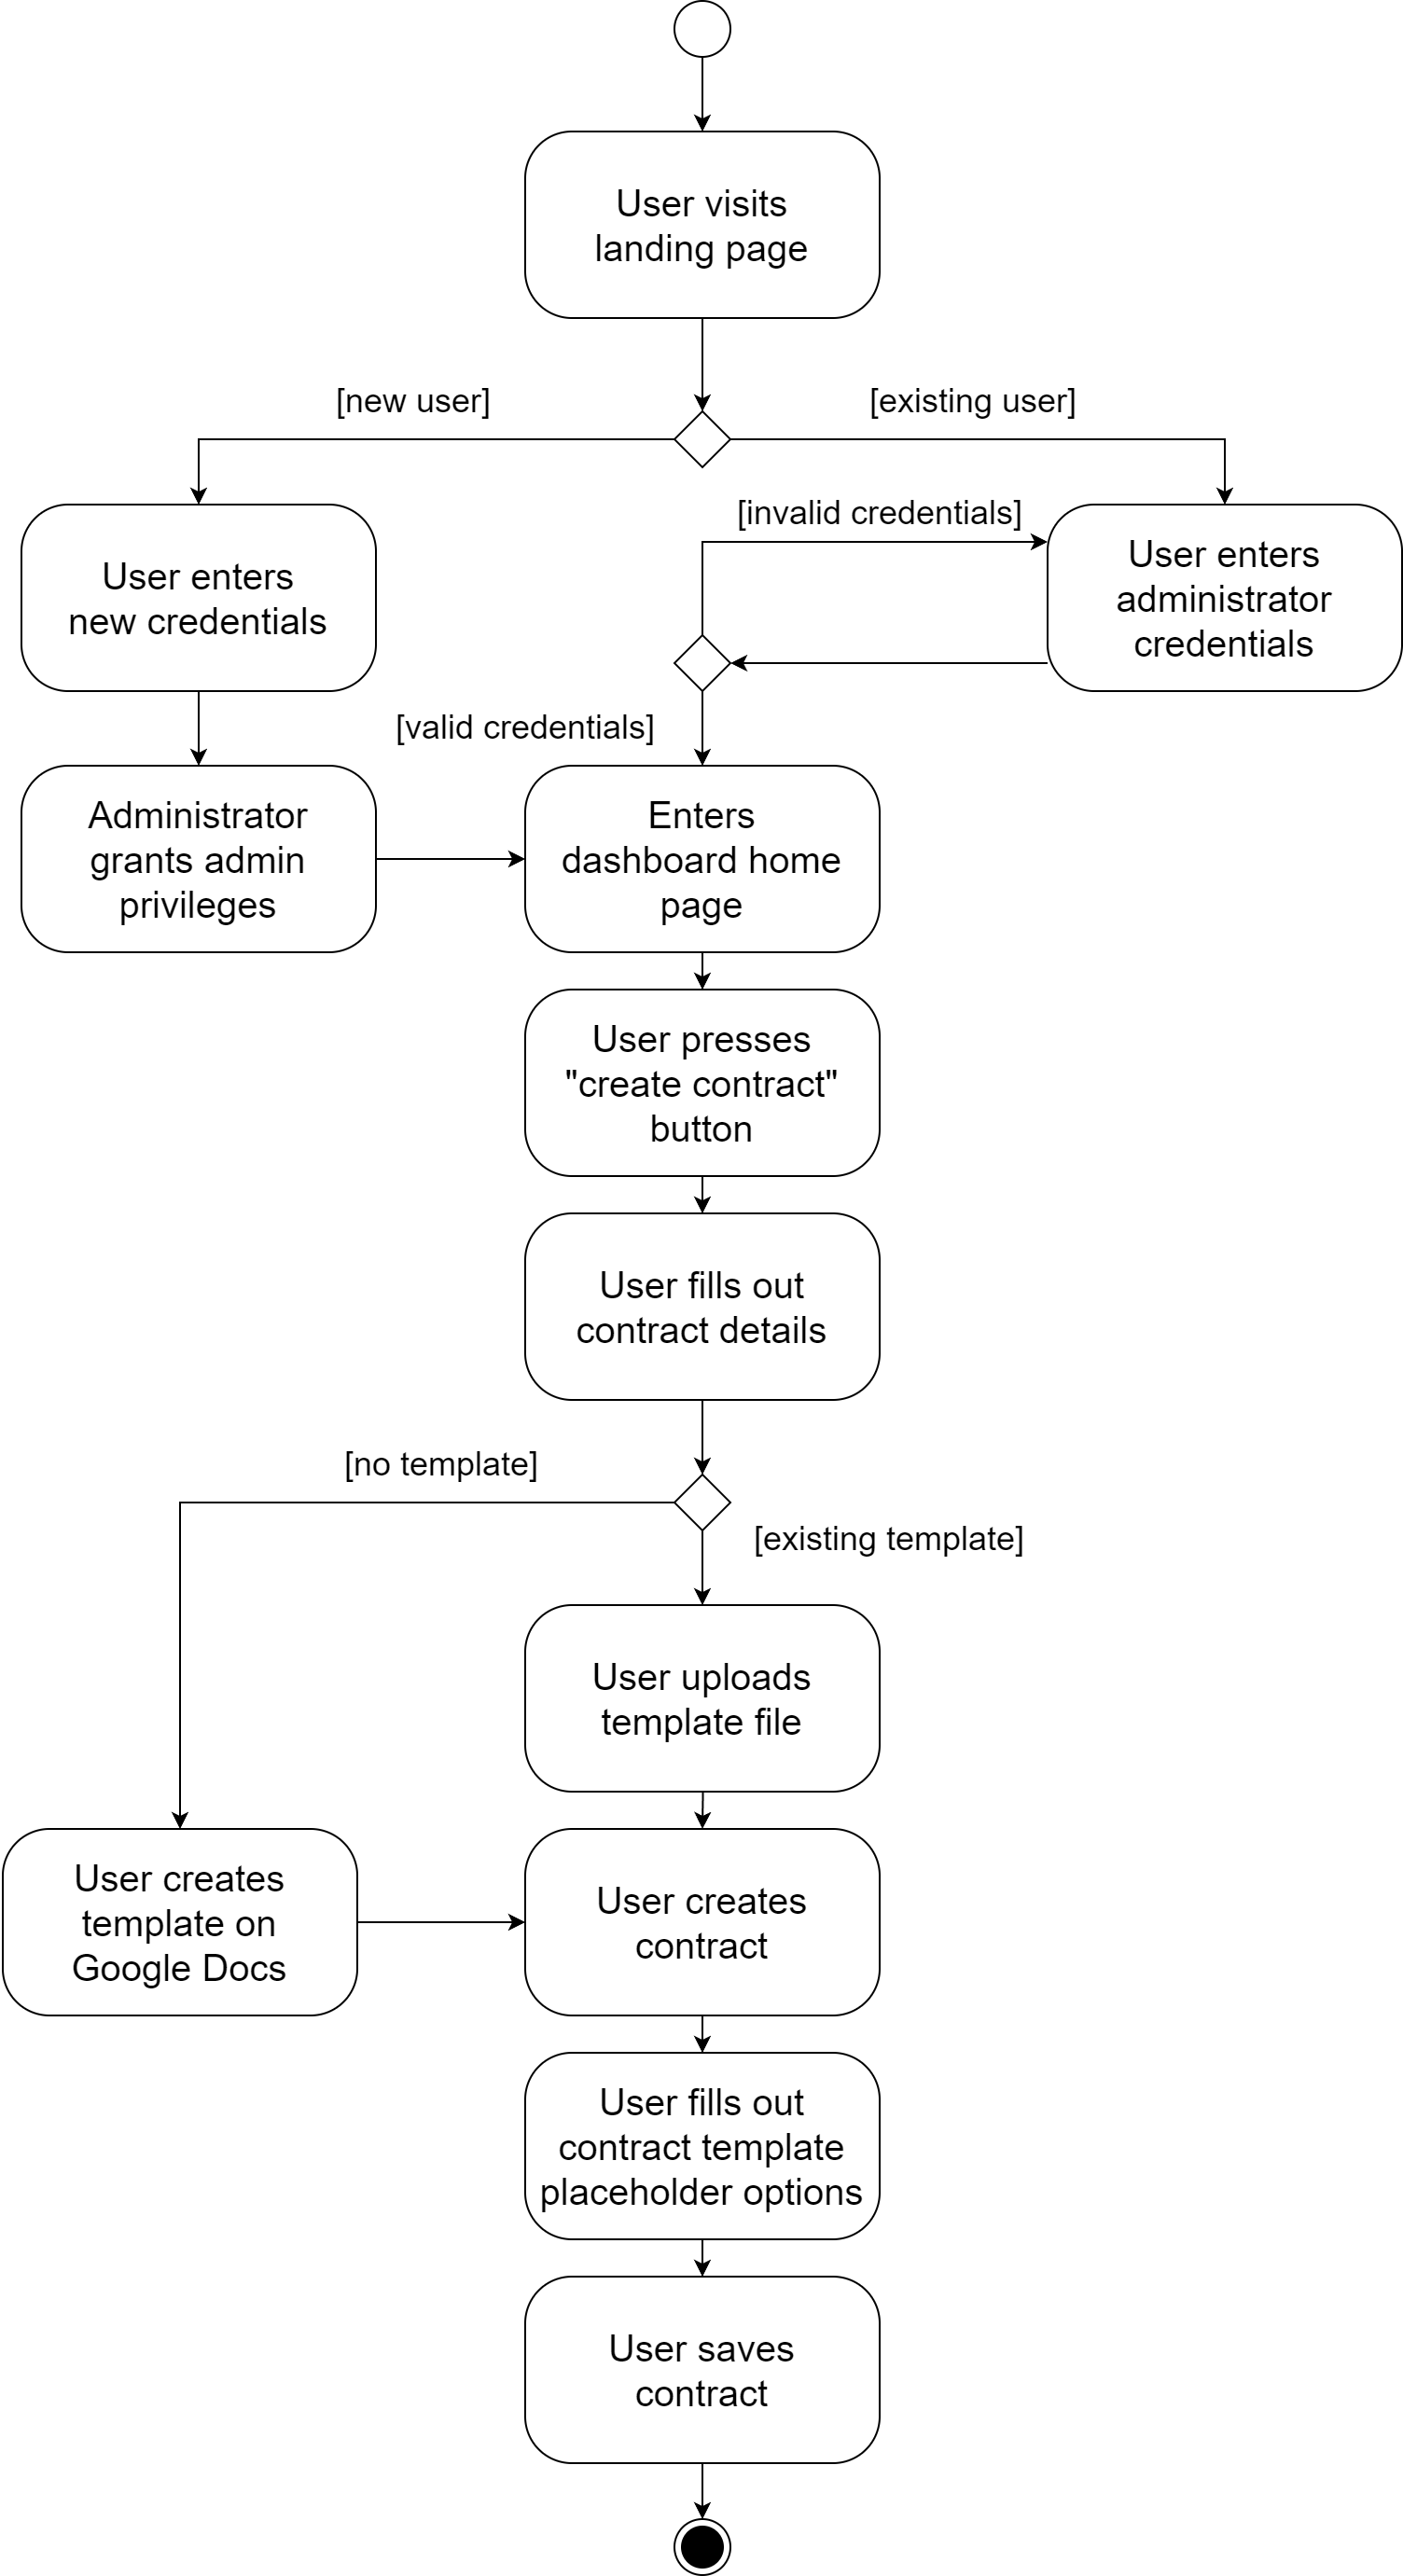
\includegraphics[scale=0.2]{images/software/activity.png}
	\caption{A szerződések létrehozásának activity diagramja}
        \label{software:activity}
\end{figure}

A \ref{software:activity}. ábrán látható a szerződések létrehozásának activity diagramja. A tevékenység kezdetén a felhasználó meglátogatja a weboldal főoldalát.

A weboldal főoldalából két lehetőség nyílik a felhasználó fele: Ha a felhasználó már rendelkezik egy adminisztrátor fiók hitelesítési adataival, akkor beírhatja ezeket a hitelesítési adatokat. Hogyha a rendszer helyesnek véli ezeket az adatokat, akkor továbbengedi a műszerfal kezdőlapjára. Ha viszont a rendszer helytelennek gondolja a hitelesítési adatokat, a felhasználó újból be kell írja azokat.

Ha nincsen adminisztrátor fiókja a felhasználónak, akkor létrehoz egy új fiókot, új hitelesítési adatok megadásával. A hitelesítési adatok megadása után megvárja, hogy egy másik adminisztrátor adminisztrátor jogokkal ruházza fel őt. Ezután kerül át a felhasználó a műszerfal kezdőlapjára.

Miután a felhasználó a műszerfal kezdőlapján van, rákattint a "Szerződés létrehozása" gombra. Ezután kitölti a szerződés sablon összes részletét. Hogyha a felhasználó már készült egy előre elkészített sablonnal, akkor feltöltheti azt. Ha nem készült már előre elkészített sablonnal, akkor a felhasználó létrehoz egy új, üres sablont a Google Docs-ban.

Miután létrejött a dokumentum sablonját, a felhasználó létrehozza a szerződéstípust. A szerződéstípus létrehozása után a felhasználó kitölti az összes olyan űrlapopciót, amelyet a felhasználó megváltoztathat, és amely a Google Docs rendszerben létrehozott dokumentumsablonon megtalálható.

Az űrlapopciók létrehozása után a felhasználó lementi a szerződés típusát, a folyamat végére érve.

\pagebreak

\section{Végleges szerződések kigenerálása}

\begin{figure}[!h]
	\centering
        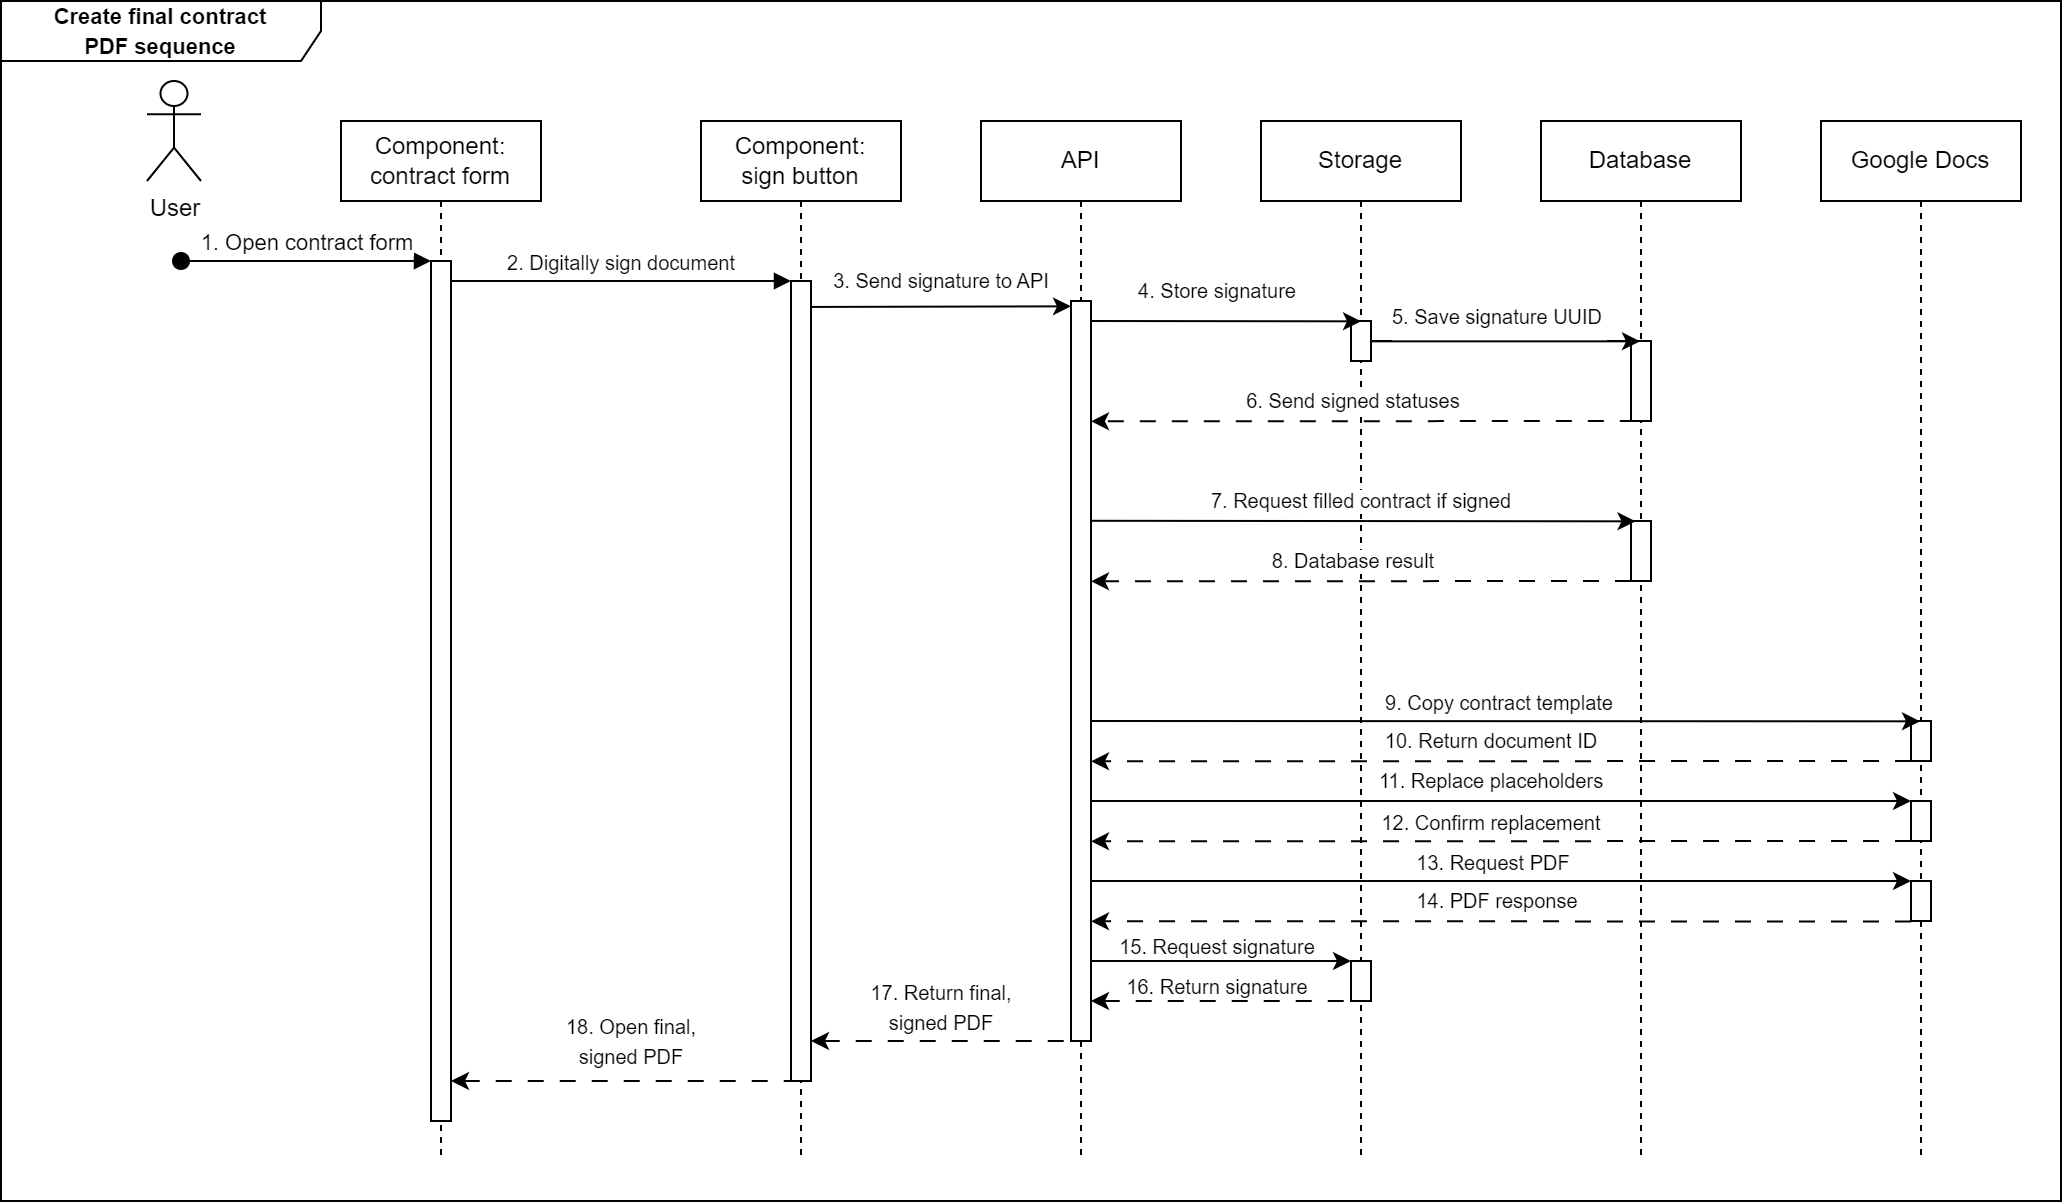
\includegraphics[scale=0.22]{images/software/sequence.png}
	\caption{A végleges szerződések kigenerálásának szekvencia diagramja}
        \label{software:sequence}
\end{figure}

A \ref{software:sequence} ábrán látható a végleges szerződések kigenerálásának szekvencia diagramja. Ebben a szekvenciában hét alkomponens játszik szerepet: maga a felhasználó, a szerződés űrlapja, az aláíró gomb, az API backend, a háttértároló, az adatbázis illetve a külső Google Docs rendszer.

A folyamat elején a felhasználó kinyitja a szerződés űrlapját, és a szerződés űrlapján rákattint az aláíró gombra. A dokumentum így digitális aláírásra kerül. Az aláíró gomb elküldi a digitális aláírást az API számára, amely továbbküldi azt a háttértárolónak. A háttértároló kigenerál egy egyetemesen egyedi azonosítót, ami jellemzi az adott digitális aláírást, és elküldi az adatbázisnak. Az adatbázis visszatéríti az API-nak, hogy mely felhasználók írták eddig alá a szerződést és melyek nem.

Ha az összes felhasználó aláírta a szerződést, akkor folytatódik a végleges szerződés kigenerálása. Az API kér egy másolatot a szerződés sablonáról a Google Docs rendszertől. A Google Docs visszaszolgáltatja az új másolat azonosítóját. Az API ezután összegyűjti az összes űrlap elemet, amelyet helyettesíteni szeretne a dokumentumon. Ezeket a helyettesíteket kötelegelve elküldi a Google Docs rendszernek. A Google Docs visszaküldi a kicserélt űrlapelemek számát az API-nak. Ezután az API megkéri a Google Docs rendszertől, hogy generáljon egy PDF dokumentumot. A Google Docs rendszer visszatéríti az API-nak a kitöltött PDF dokumentumot.

A kitöltött PDF dokumentum még nincs aláírva. Az API lekéri a háttértárolóból a digitális aláírásokat. A háttértároló visszaszolgáltatja az API-nak ezeket az aláírásokat. Az API beszúrja a PDF dokumentumba a \textit{pdf-lib}
és \textit{node-signpdf} könyvtárak segítségével a digitális aláírásokat, kigenerálja az AVDH tanúsítványokat, és visszatéríti a végleges, digitálisan aláírt PDF állományt az aláíró gombnak, ahonnan visszakerül a szerződési űrlapra, és kinyílik a felhasználó számára, hogy megtekintse.

\section{Felhasználói felület tervezése}

\begin{figure}[!h]
	\centering
        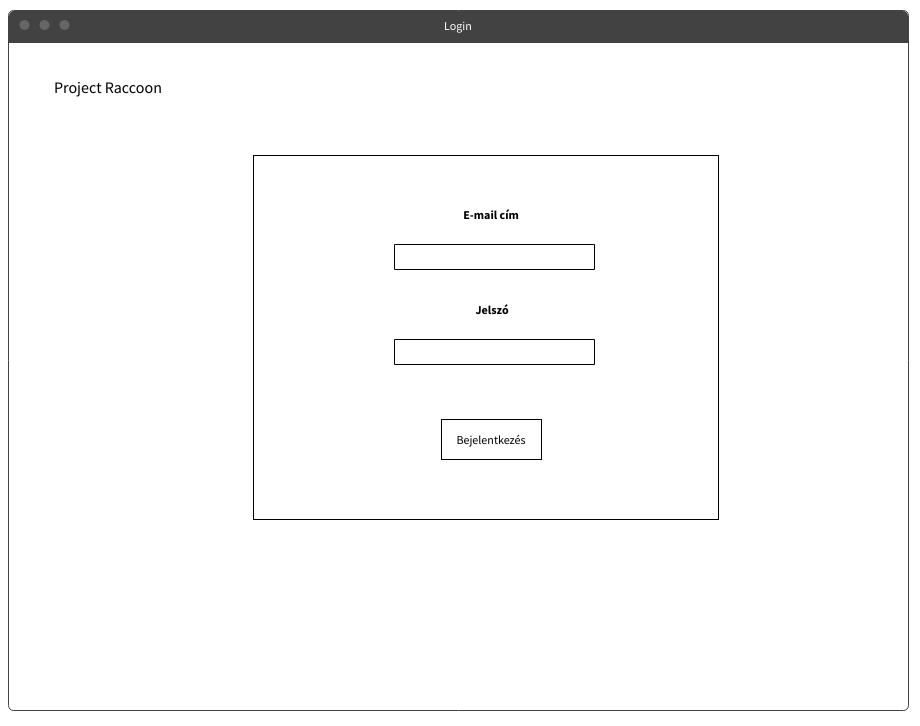
\includegraphics[scale=0.5]{images/wireframe/login.png}
	\caption{A Project Raccoon belépési felületének drótváza}
        \label{wireframe:login}
\end{figure}

A következőekben a tervezés során kialakított drótvázról (\textit{wireframe}) lesz szó. Ezen \textit{wireframe}k segítségével átfogó képet kaphatunk a felületek kinézetéről, az elemensek elhelyezkedéséről, egymáshoz való viszonyulásáról és méretéről. Mindezt anélkül, hogy az apró részletek, színek elhomályosítanák ezen nagyobb körvonalakat. A tervezés során elsődleges szempont volt a felület könnyű használhatósága, az átláthatóság és a reszponzivítás. A folyamat során igyekeztünk betartani Nielsen által felsorolt heurisztikákat \cite{nielsen2005ten} a felület minél nagyobb fokú használhatóságának érdekében. 

\begin{figure}[!h]
	\centering
        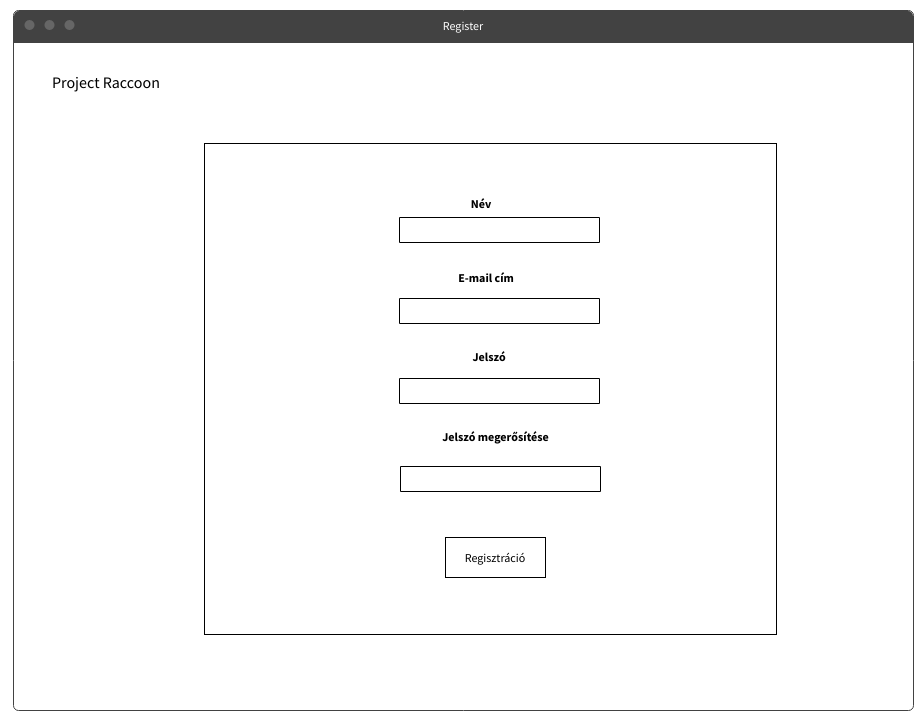
\includegraphics[scale=0.5]{images/wireframe/register.png}
	\caption{A Project Raccoon regisztrációs felületének drótváza}
        \label{wireframe:register}
\end{figure}

Tekintsünk meg néhány fontosabb oldal \textit{wireframe}jét. A bemutatott dizájn az átlagfelhasználók szemszögéből fogja bemutatni a weboldalt (tehát eltekintünk most az adminisztrátori jogkörrel ellátott felhasználóktól). Legelsőnek a \ref{wireframe:login}. ábrán láthatjuk a bejelentkezési oldal drótvázát, amely egyszerűen csak a felhasználót hitelesítő adatok beírása végetti szövegdobozokat és a belépéshez szükséges gombot tartalmazza középre igazítva. A belépéshez egy email cím és egy jelszó szükséges. Miután a felhasználó ezeket beírta, a ``Bejelentkezés'' gombra kattintva be tud lépni a platformra és megtekintheti a saját \textit{dashboard}ját.

Amennyiben a felhasználó nem rendelkezik fiókkal, regisztrálhat a regisztrációs felületen, amely a következőképp néz ki (\ref{wireframe:register}. ábra). A felület tartalmaz négy szövegdobozt, amelybe a felhasználó beírhatja adatait ezek rendre a következőek: név, email cím, jelszó és a jelszó újbóli beírása - az elgépelések kivédéséért fontos. Ezután pedig egy ``Regisztráció'' gomb következik a beírt szövegek elküldése és a regisztráció finalizálása végett. 

\begin{figure}[!h]
	\centering
        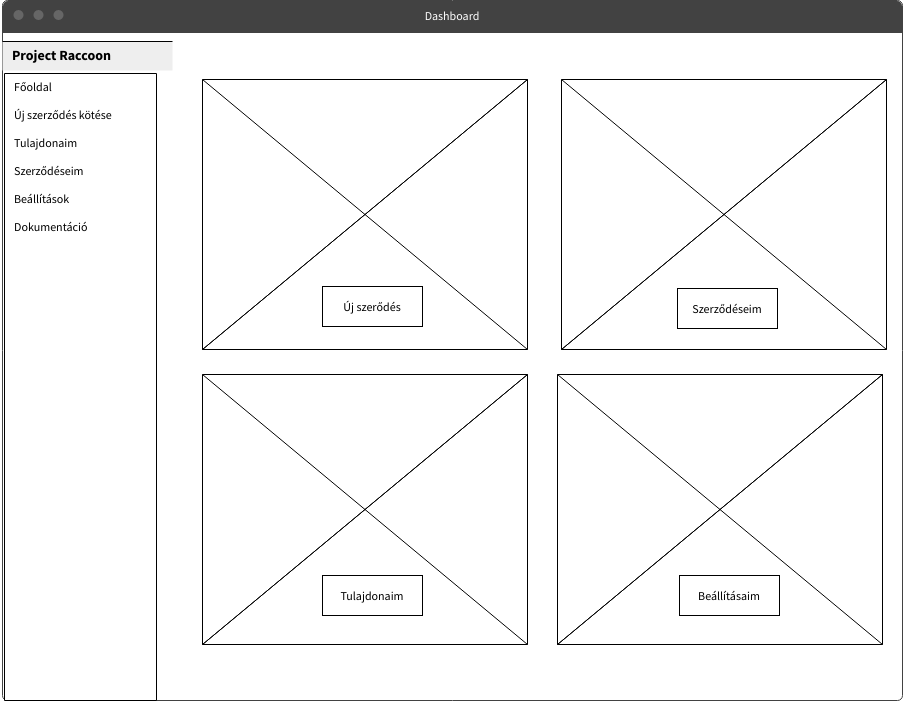
\includegraphics[scale=0.5]{images/wireframe/dashboard.png}
	\caption{A Project Raccoon \textit{dashboard}jának drótváza}
        \label{wireframe:dashboard}
\end{figure}

Sikeres regisztráció után a felhasználó be tud lépni a bejelentkezési felületen. Miután ez megtörtént, megtekintheti a \textit{dashboard}ját, amely a tervezési fázisban a következőképp nézett ki. Ezt a \ref{wireframe:dashboard}. ábra is szemlélteti. Bal oldalt található egy menü, amely segítségével a felhasználó navigálhat a weboldalon: létrehozhat új szerződést, megtekintheti a tulajdonait, valamint a szerződéseit. Különböző beállításokat végezhet, mint például: adatai módosíthatja, vihet be új adatokat, amelyek szükségesek lehetnek a szerződések kitöltése érdekében, de nem voltak elkérve a regisztráció során (anyja születési neve, személyi igazolványának száma, lakhelye stb.). Illetve megtekintheti a platform dokumentációját, vagyis a súgót (használati kézikönyv) - ha bármilyen problémája akad a felhasználónak az oldal használata közben, többek között könnyedén megkeresheti a megoldást/informálódhat ebből is. Ez növeli a felhasználók kényelmét, és az önálló használatot. Tanulmányok már 2013-ban kimutatták, hogy az emberek szívesebben választanak önálló segítségkérési lehetőségeket, mintsemn emailt írjanak, hívást kezdeményezzenek egy ügyfélszolgálattal, illetve, hogy ``a felhasználók 70\% elvárja, hogy egy portálon igénybe tudjanak venni olyan segítséget, amelyhez nem kell más ember beavatkozása'' \cite{van2013self}. Végezetül pedig egy ``Főoldal'' menüpont is szerepel, amely visszavisz a \textit{dashboard}ra. A navigációs menü felett található a platform neve is, amely megjelenik ugyanúgy belépéskor és regisztrációkor is. Jelenleg ezt egy egyszerű \textit{``Project Raccoon''} felirat szemlélteti. 

Középre helyezve pedig megtalálhatóak ugyanezek a főbb alpontok, csupán nagyban kiemelve, hogy még szembetűnőbbek legyenek a felhasználók számára.  

\begin{figure}[!h]
	\centering
        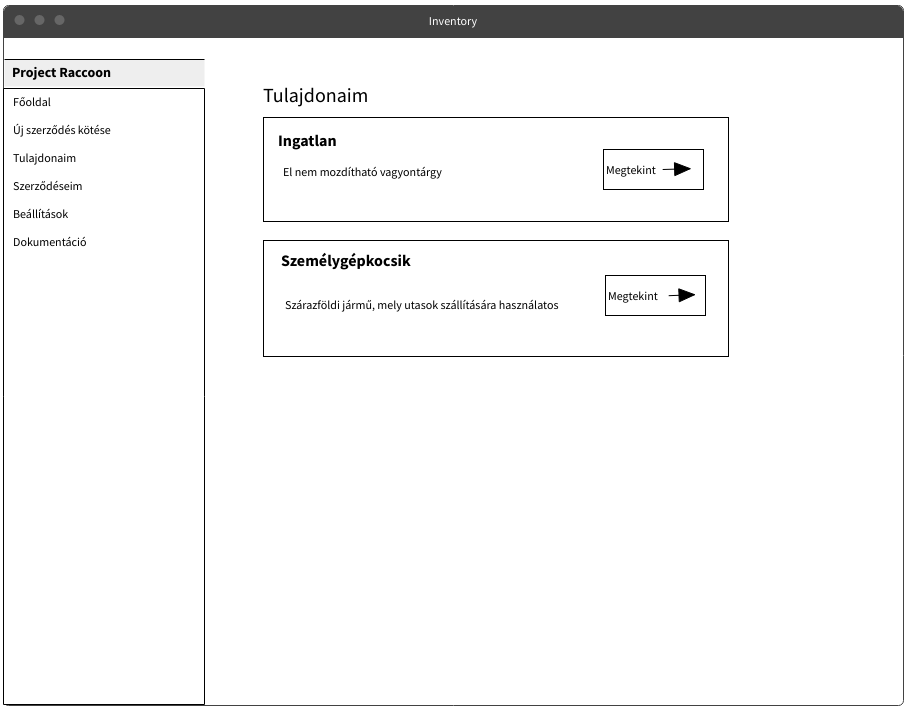
\includegraphics[scale=0.4]{images/wireframe/inventory.png}
	\caption{A Project Raccoon tulajdonokat (kategóriánként) megjelenítő felületének drótváza}
        \label{wireframe:inventory}
\end{figure}

A következő \ref{wireframe:inventory}. ábrán a ``Tulajdonaim'' oldalt láthatjuk, amely a portál adatbázisába felvitt ingó és ingatlanokat listázza. Oldalt a már elmagyarázott navigációs menü található, középül pedig a két kategóriára osztott tulajdonok. Ezek megnevezései alatt egy rövid leírás található az adott katergóriáról, illetve egy-egy gomb, ami még részletesebb megtekintését/listázását adja az adott tulajdonoknak.

A fontosabb wireframek közül utolsónak a szerződéseket listázó oldalt tekintsük meg. A \ref{wireframe:contracts}. ábra ezt szemlélteti. Bal oldalt a fentebb elmagyarázott navigációs sáv található, középül pedig a szerződések típusai szerint kategóriákra osztva láthatjuk és menedzserelhetjük a szerződéseinket. Ezalatt értjük új szerződések kitöltését/létrehozását, amelyet a kategórián belüli ``Új szerződés kitöltése'' gombra kattintva meg is tehet a felhasználó.

\begin{figure}[!h]
	\centering
        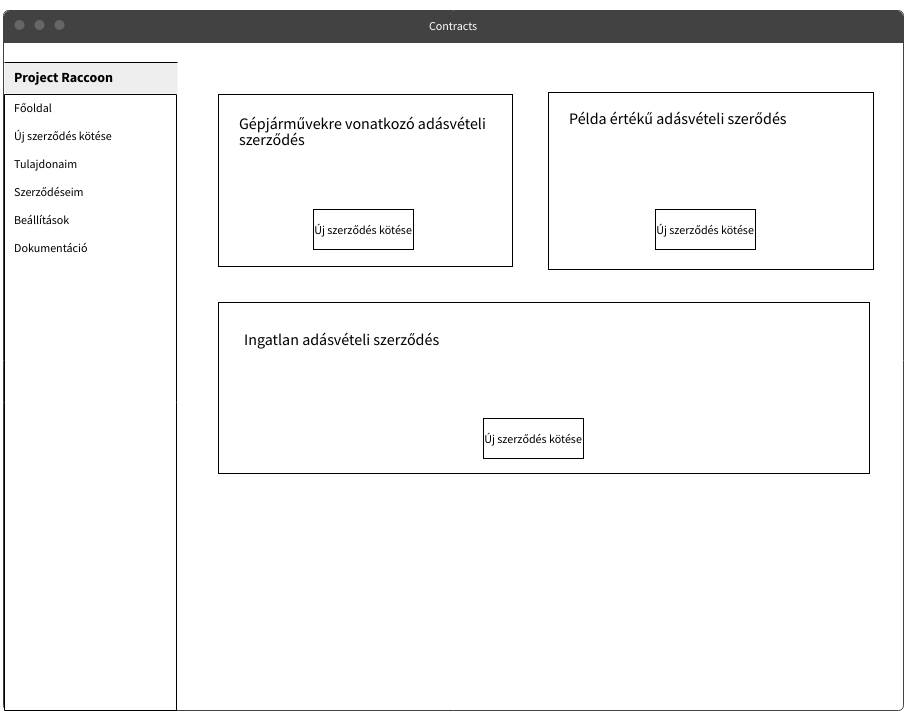
\includegraphics[scale=0.5]{images/wireframe/contracts.png}
	\caption{A Project Raccoon szerződéseket listázó felületének drótváza}
        \label{wireframe:contracts}
\end{figure}

Az eddigi példákból látható, hogy a tervezést a minél egyszerűbb használat, a letisztult design valamint a hatékony haszálhatóság vezérelte. A következő, \ref{chapter4}. fejezetben részletesebben kitértünk a megvalósítás részleteire, a felületek megvalósítására.

\section{Felhasználói use case-ek}

\begin{figure}[!h]
	\centering
        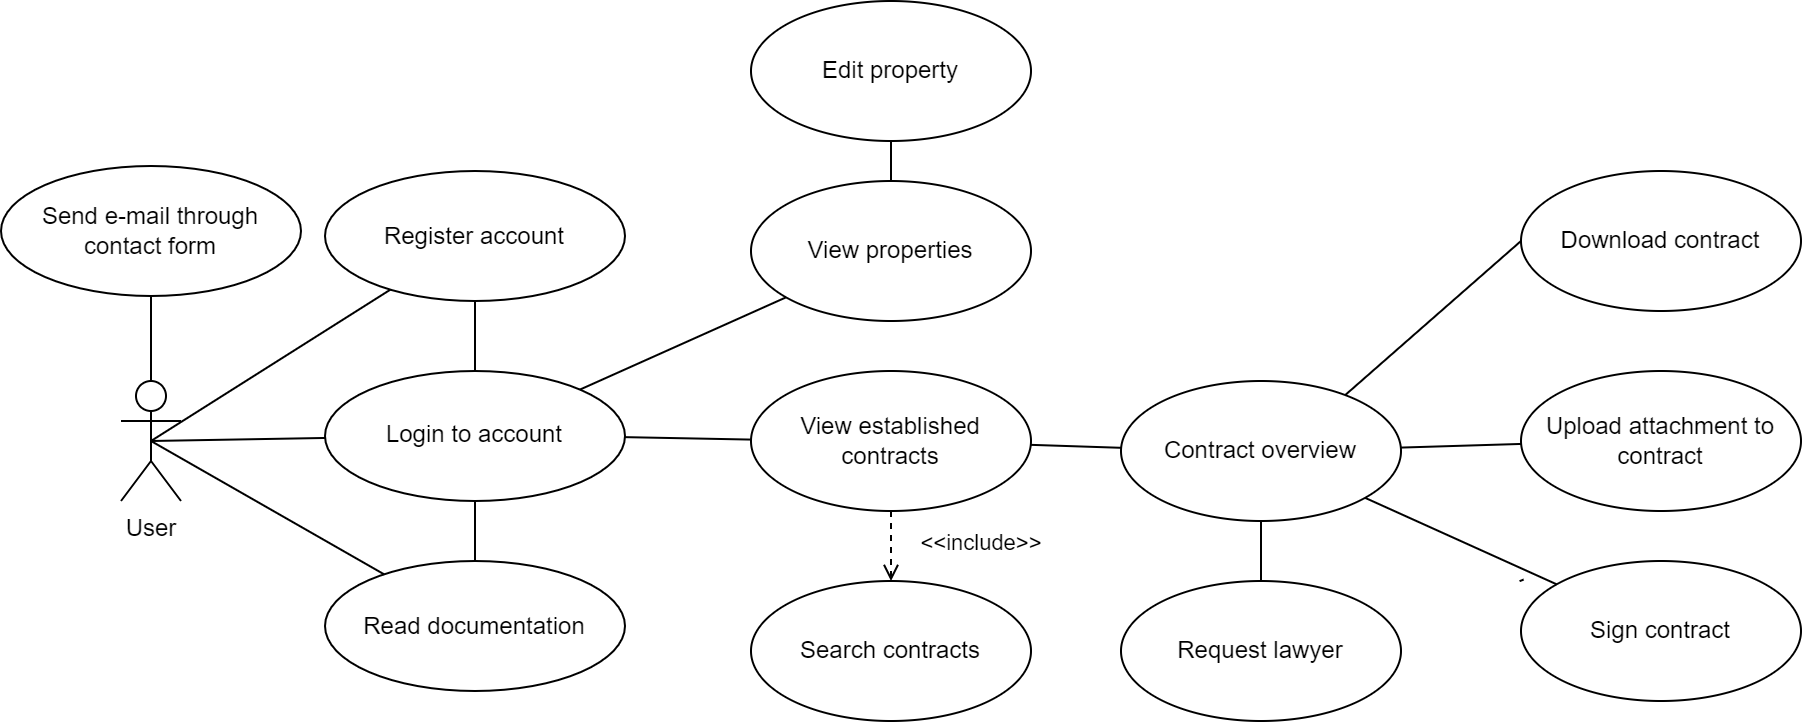
\includegraphics[scale=0.25]{images/software/user-use-case.png}
	\caption{A hitelesített felhasználók use case diagramja}
        \label{software:userusecase}
\end{figure}

A \ref{software:userusecase}. ábrán látható az összes funkcionalitás, amelyre jogosultak a felhasználók. Mivel nagyon sok funkcionalitás van, az ábrán egy leegyszerűsített diagram látható. Kezdeti fázisban, mikor a felhasználó a főoldalon van, küldhet egy e-mail-t a weboldal adminisztrátorainak egy kapcsolatfelvételi űrlapon keresztül, készíthet egy saját fiókot, beléphet egy már létező fiókba, vagy megtekintheti a felhasználók számára készített kézikönyvet.

A belépés után a felhasználók megnézhetik a meglévő szerződéseiket vagy megtekinthetik a saját tulajdonaikat. A saját tulajdonaik megtekintése közben az egyes tulajdonokat szerkeszteni is tudják. A szerződések megtekintése közben kereshetnek a szerződések között, vagy akár megtekinthetnek egy meglevő szerződést.

A meglévő szerződések megtekintése során a felhasználók kérhetnek ügyvédet a szerződés ellenőrzésére, letölthetik a szerződést, amennyiben mindenki aláírta, feltölthetnek mellékleteket egy nem véglegesített szerződés keretén belül, vagy aláírhatják a szerződést.

A \ref{software:contractdownload}. táblázatban az egyik legfontosabb use case: a szerződések letöltésének kiterjesztett magyarázatát láthatjuk.

\begin{longtable}{|p{0.35\textwidth}|p{0.55\textwidth}|}
\caption{Felhasználási eset: Szerződés letöltése}
\label{software:contractdownload}
\hline
\multicolumn{2}{|c|}{\textbf{Felhasználási eset}} \\
\hline
\textbf{Felhasznási eset száma:} & PR-1 \\
\hline
\textbf{Felhasznási eset leírása:} & Egy felhasználó letölti az egyik szerződése véglegesített, kitöltött PDF verzióját. \\
\hline
\textbf{Előfeltételek:} & 
\begin{enumerate}[itemsep=0pt,parsep=0pt,topsep=0pt,partopsep=0pt]
    \item A felhasználónak be kell jelentkeznie.
    \item A szerződés összes  kell lennie.
    \item A szerződést minden félnek alá kell írnia, beleértve az ügyvédeknek is.
    \item A felhasználónak hozzáférése kell legyen a szerződéshez.
\end{enumerate} \\
\hline
\textbf{Alapfolyamat:} & 
\begin{enumerate}[itemsep=0pt,parsep=0pt,topsep=0pt,partopsep=0pt]
    \item A felhasználó bejelentkezik a kezelőfelületre.
    \item A felhasználó listázza az összes szerződését, majd a kívánt szerződésre kattint, legyen az manuális kereséssel vagy a "Szerződések keresése" felhasználási esettel.
    \item A felhasználó rákattint a "Szerződés letöltése" gombra.
    \item A szerződés letöltődik a felhasználó számítógépére PDF fájlként.
\end{enumerate} \\
\hline
\end{longtable}

\begin{figure}[!h]
	\centering
        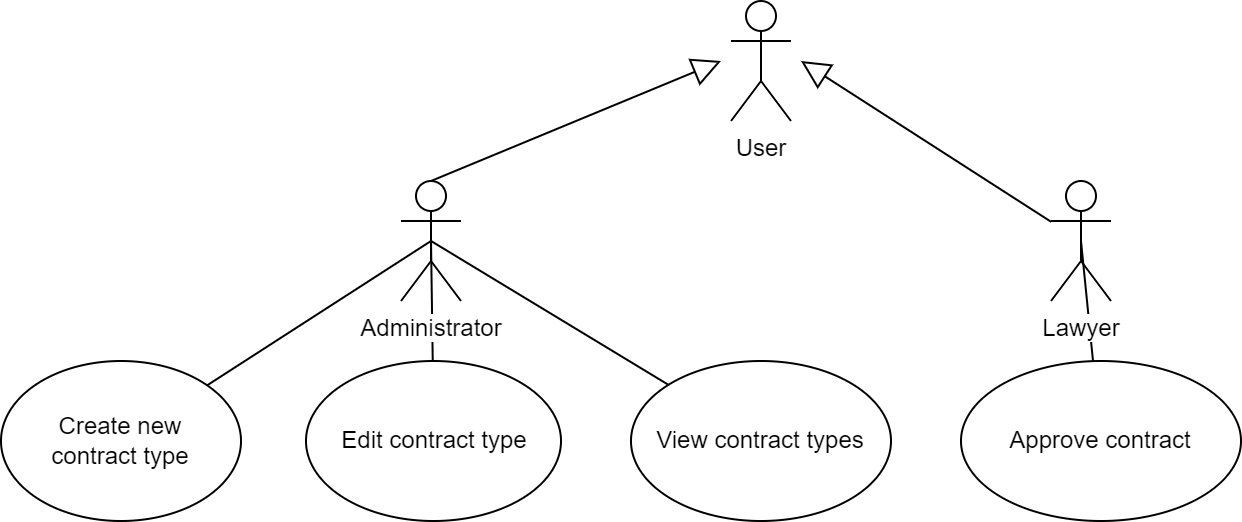
\includegraphics[scale=0.33]{images/software/special-use-case.png}
	\caption{A speciális felhasználók use case diagramja}
        \label{software:specialusecase}
\end{figure}

A \ref{software:specialusecase}. ábrán látható a speciális felhasználók számára elérhető funkcionalitások. Mivel az adminisztrátorok és az ügyvédek egyaránt felhasználók, mindenre képesek, amire a rendes felhasználók is képesek.

Az ügyvéd felhasználók alá tudják írni azokat a szerződéseket, amelyre meghívták őket, illetve az adminisztrátorok képesek létrehozni új szerződés típusokat, ki tudják listázni és meg tudják módosítani egyenként őket.

\pagebreak